\documentclass[12pt]{article}
\usepackage{fullpage}
\usepackage{graphicx, rotating, booktabs} 
\usepackage{times} 
\usepackage{fbb} 
\usepackage{natbib} 
\usepackage{indentfirst} 
\usepackage{setspace}
\usepackage{grffile} 
\usepackage{hyperref}
\usepackage{tikz-cd}
 \usetikzlibrary{cd}
\usepackage[export]{adjustbox}
\usepackage[most]{tcolorbox}
\usepackage{verbatimbox}
\usepackage{lscape}
\usepackage{afterpage}
\usepackage{amsmath}
\usepackage[labelfont={bf},textfont=it,labelsep=period]{caption}
 \usepackage{multirow} 
\setcitestyle{aysep{}}
\usepackage{dcolumn}

\hypersetup{
  colorlinks = true,
  urlcolor = blue,
  linkcolor = black,
  citecolor = black,
  pdfauthor = {Joshua Alley},
  pdfkeywords = {},
  pdftitle = {},
  pdfsubject = {},
  pdfpagemode = UseNone,
%  pdffitwindow = true
%  pdfcenterwindow = true
}



\singlespace
\title{\textbf{Using Hierarchical Models to Estimate Heterogeneous Effects}}
\author{Joshua Alley \\
Assistant Professor \\
Baylor University \\
Joshua\_Alley@baylor.edu
}

 
\date{\today}

\bibliographystyle{apsr}

\usepackage{sectsty}
\sectionfont{\Large}
\subsectionfont{\noindent\large\textit}
\subsubsectionfont{\normalsize}

\makeatletter
\renewcommand\tiny{\@setfontsize\tiny{9}{10}}
\makeatother


\begin{document}

\maketitle 

\begin{abstract} 
%Heterogeneous effects are common in social science. 
This note describes why, when, and how to use Bayesian hierarchical models to estimate heterogeneous effects. 
While an ample literature suggests that hierarchical models provide helpful regularization and information about effect variation, political scientists rarely use them to estimate heterogeneous effects. 
Doing so is simple, however. 
To start, identify potential sources of heterogeneity. 
Then, fit a hierarchical model with two linked regressions, one connecting treatment with the outcome, and another that models the treatment effects with potential sources of heterogeneity partially pools individuals.
This captures systematic group-level variation and random individual variation in heterogeneous effects, encompasses the diversity of interactions in theories, and fits commonly used modeling frameworks. 
Hierarchical modeling is more flexible than linear interactions and reduces the risk of underpowered subgroup comparisons.
It also provides a more interpretable framework for testing theories than machine-learning tools. 
I document these claims with a simulation analysis and extension of a published study. 
Researchers can thus use hierarchical models alongside other approaches to understand heterogeneous effects for scholarship and policy.
\end{abstract} 


\newpage 
\doublespace 


\section{Introduction}


% one: het effects matter
Whether in observational or experimental studies, every independent variable social scientists examine impacts some units differently than others. 
Common estimands aggregate heterogeneous effects.\footnote{For instance, \citet{Abramsonetal2022} note that the average marginal component effect (AMCE) of conjoint experiments gives more weight to intense preferences.} 
Such average effects are useful, but they often obscure interesting and important variation. 


Understanding heterogeneous effects is essential for policy and scholarship. 
Estimating heterogeneity allows scholars to clarify when their independent variable most or least impacts some outcome.
Policymakers can maximize the impact of finite resources with targeted interventions, for example by providing job training to individuals who are more likely to benefit. 
% expand/sharpen this, if there is space. (There is not for PA) 

% two: introduce my solution 
This paper explains why, when and how to use hierarchical models to estimate heterogeneous effects. 
A large statistics literature suggests that Bayesian hierarchical models are a useful tool for  heterogeneous effects estimation (e.g., \cite{FellerGelman2015, McElreath2016, Dorieetal2022}).
Political scientists tend to rely on interactions or machine learning tools instead, however.  
For instance, of the three applied political science citations of \citet{FellerGelman2015}, only \citet{Marquardt2022} models treatment effects. 


% power problems
This oversight matters because there are few tools that are well-suited to test the proliferation of conditional arguments in the social science. 
Social scientists often propose conditional theories \citep{ClarkGolder2023} and are interested in how different people respond to the same stimulus for normative or policy reasons.
Many theories proposing a singe modifier for the same relationship and interest in diverse subgroups suggest that multiple modifiers are the rule, not the exception.  
For example, scholarship on audience costs has considered how foreign policy dispositions \citep{KertzerBrutger2016}, partisanship \citep{LevenduskyHorowitz2012}, gender \citep{Barnhartetal2020, SchwartzBlair2020} and policy preferences \citep{Chaudoin2014} modify individual reactions to a leader backing down from a threat.
Such a multiplicity of theoretically informed modifiers complicates empirical testing, however. 


Scholars cannot ignore heterogeneity, but the most common tools either increase the risk of spurious results or are hard to interpret and use. 
Interaction terms and subgroup analysis are perhaps the most common tool, but can mislead. 
Simple interactions and subgroup analyses are ubiquitous because they are relatively easy to interpret, but these have serious power concerns. 
Many political science analyses have low power even to detect main effects \citep{ArelBundocketal2022}.
Adequate power for estimates of even a single interaction can require significantly more data \citep{Gelman2018}, which may be prohibitively expensive or impossible.
As a result, statistically significant heterogeneous effect estimates may be far too large--- the result of noise in the data, not systematic differences. 
This problem is partially responsible for widespread issues replicating findings based on interactions \citep{Simmonsetal2011}. 


Scaling up the number of modifiers is therefore something that theory suggests scholars should do, but doing so with interactions is not easy. 
The interpretation benefits of parametric interactions diminish as the number of modifiers increase- the different terms in interactions of three or four variables can be difficult to parse.
It also further raises the risk of spurious inferences due to power concerns and picking up noise in ever more finely sliced subgroups.


% three: loads of techniques
Given multiple sources of heterogeneity, machine-learning tools such as random forests \citep{GreenKern2012, WagerAthey2018}, support vector machines \citep{ImaiRatkovic2013}, and ensemble methods \citep{Grimmeretal2017, Kuenzeletal2019, Dorieetal2022} are more likely to avoid over-fitting.
These machine learning algorithms usually have some regularization component and can discover complex patterns and high-dimensional variation across multiple modifiers.\footnote{\citet{BlackwellOlson2022} describe a lasso approach to interactions that sits between machine learning and linear regressions.}
These tools can be difficult to interpret and implement, especially in smaller social science datasets. 
A lack of interpretability is especially problematic for testing the relative weight of multiple modifiers. 


The hierarchical strategy I propose here addresses the problems of interactions with regularization, and issues of interpretation in machine learning.
I do this by showing how scholars can use two connected regressions to estimate theoretically informed models of multiple heterogeneous effects.
Using hierarchical models is more flexible than standard interactions but easier to implement and interpret than machine learning approaches.  
It preserves a straightforward structure while accommodating more factors and ameliorating the downsides of subgroup analysis. 
This facilitates argument testing.
The main downside is that unlike machine learning, the hierarchical approach lacks the flexibility to discover high-dimensional heterogeneity.  
Hierarchical modeling therefore works best when theory indicates more than two modifying factors and there is less emphasis on discovery.\footnote{\citet{Goplerud2021} introduces a model that uses Bayesian structured sparsity to estimate which group coefficients are similar and which are different. In this approach, researchers use theory to inform potential groups, but the data determines common estimates for groups.} 


There are two key steps when theory and data make using hierarchical models worthwhile.
First, researchers should identify potential modifiers of a treatment, and determine the most theoretically appropriate model of treatment effects. 
Second, they should take that model of treatment effects and connect it to a model with individual effects linking a treatment and outcome.
Modeling heterogeneous effects in this way produces interpretable results, which facilitates argument testing.
It also allows researchers to compare different sources of heterogeneous effects and describe how much an effect varies.  


While frequentist estimation of hierarchical models is possible, Bayesian estimation is straightforward and more informative.
Bayesian estimation provides crucial information by connecting parameters through common prior distributions, thereby regularizing estimates and propagating uncertainty. 
Working with posterior distributions also gives researchers more flexibility to describe how and when effects vary. 
While computation and coding were once a barrier to employing Bayesian methods, fitting a wide range of hierarchical models is straightforward with the brms package in \textsf{R} \citep{Buerkner2017}.\footnote{I provide example code in this note and the appendix.}
%Calculating substantive effects is also simple \citep{ArelBundockme}.



% wrap and introduce the application 
In the remainder of this paper, I describe how and when to estimate hierarchical models of heterogeneous effects.
I then employ a simulation study to compare OLS and hierarchical estimates of individual treatment effects under different conditions.
Finally, I demonstrate the process by analyzing a study of how military alliances shape public support for war by \citet{TomzWeeks2021}. 
The reanalysis reveals that alliances increase support for intervention most among white men who support international engagement but are otherwise skeptical of using force. 
%Alliances increase mass support for war by impacting individuals who otherwise prefer peaceful collaboration. 



\section{Hierarchical Modeling of Heterogeneous Effects}


There are two steps in hierarchical models of heterogeneous effects. 
First, researchers must identify potential sources of heterogeneity, and think about the right model of how those factors shape heterogeneity.
This will also depend on what variation is most important and interesting. 
Theory, policy concerns, or normative factors are all possible motivations. 


This first step determines what heterogeneous effects a researcher estimates. 
It is analogous to researchers thinking through their regression specifications--- the same sort of care should go into the sources of heterogeneity. 
Researchers need to define what variation is most important, links heterogeneous effects to theory, and structures modeling.\footnote{It also facilitates pre-registration when applicable.}
Not thinking carefully about sources of heterogeneity will obfuscate results and can hinder model fitting.
   

% three ways to set groups
There are three general approaches to defining groups.  
First, researchers can set groups using combinations of other treatments, especially when an intervention has several dimensions but theory emphasizes one of them. 
The experimental design determines modifiers, and the model estimates heterogeneous treatment effects.   
If researchers want to know how different issues shape the impact of elite foreign policy cues \citep{GuisingerSaunders2017}, they could include indicators of issues, for instance.
Hierarchical estimators for topic-sampling experiments estimate how a treatment effect varies across different topics \citep{CliffordRainey2023}. 


Researchers sometime use fully crossed regression interactions to estimate the impact of a treatment across experimental strata, but this approach risks spurious results by functionally estimating subgroup results, most of which do not have adequate power. 


A second approach uses unit, demographic and contextual factors to estimate effect heterogeneity. 
Here, researchers examine what factors within or around units shape their response to an independent variable.
For example, one could use a mix of individual and state-level factors to predict divergent consequences of a survey experiment treatment. 
Other use cases include estimating how different geographic units respond to an intervention.\footnote{Extrapolation to a representative sample for such units might require poststratification.}


For example, \citet{Alley2021isq} uses alliance characteristics to examine when alliance membership increases or decreases military spending.
He models the impact of alliance participation as a function of treaty depth, partner democracy, conditions on military support, issue linkages, democratic membership, foreign policy concessions and other factors. 
All of these variables are potential sources of credibility or confounding factors.
Democratic alliances have higher depth, so this model of heterogeneity accounts for potential confounding, and finds that after accounting for depth, democracy does not impact the relationship between alliances and defense spending. 


Third, researchers might use hierarchical models to address specific policy concerns.
Policy analysts often want to know how an intervention impacts a specific population. 
Researchers might want to know if a job-training program improves employment outcomes for black women in the South, for instance.  
To do this, a researcher might specify a heterogeneous effects model with interactions of race, gender and region, plus additional controls or other factors. 


% grouping factors: numbers 
%Whether researchers use other treatments, context, or policy to determine what drives heterogeneity, group composition should depend first on the research question.
%There are some practical constraints, however.
%Using too many factors can lead to model fitting and interpretation problems by creating many small groups.
%How many factors is too many depends especially on the data- some datasets can support reasonably large groups for many factors. 
%At the other extreme, using only one grouping factor in a hierarchical model will usually add relatively little value compared to interactions. 


After defining groups, the second step is fitting a hierarchical model that links a model of the outcome with a model of heterogeneity.
Essentially, researchers model the outcome and the process that produces heterogeneous treatments. 
The model employs two connected regressions.
One regression deals with the outcome.
The other regression models the treatment effects.\footnote{If other units such as states define the groups, rather than combinations of modifying variables, then adding group-level predictors is essential. For examine, in a model where an effect varies by state, adding state-level variables like ideology, population and GDP would avoid partially pooling small groups too far towards the overall mean.}


I now briefly describe the generic hierarchical model. 
For ease of exposition, consider making between-unit comparisons based on an experimental treatment.    
Start with \textit{N} units indexed by \textit{i}, some of which receive a binary treatment \textit{T}.
Assume that the outcome variable ${y}$ is normally distributed with mean $\mu_i$ and standard deviation $\sigma$.\footnote{Researchers can and should use binary, categorical and other outcome likelihoods.}
%\textit{g} indexes two researcher-defined groups, \textit{g1} and \textit{g2}.


%The first equation predicts the outcome mean. 
The outcome for each unit depends on an overall intercept, an optional matrix of control variables \textbf{X}, and a set of individual treatment effects $\lambda_i$.
When \textit{T} is binary, estimated $\lambda$ parameters for untreated units have no impact on the outcome. 
For a continuous treatment, the impact of of treatment will depend on the product of $\textit{T}_i$ and $\lambda$.



\begin{align*}
y_i &\sim N(\mu_i, \sigma) &\text{(Likelihood)} \\
\mu_i &= \alpha + \lambda_i \textit{T} + \textbf{X} \beta &\text{(Outcome Equation)}  \\ 
\lambda_i &= \theta_i + \textbf{Z} \gamma  &\text{(Heterogeneity Equation)}\\
\theta_i &\sim N(\mu_\theta, \sigma_\theta) &\text{(Indiviudal Varying Intercepts)} 
%\gamma &\sim N(0, 1) &\text{Problem-Specific Prior} \\ 
%\beta &\sim N(0, 1) &\text{Problem-Specific Prior} \\ 
%\alpha &\sim N(0, 1) &\text{Problem-Specific Prior} \\ 
\end{align*}



%The outcome for each unit is then a function of group varying intercepts $\alpha_g$, an optional matrix of control variables \textbf{X}, and a set of group treatment effects $\theta_g$.
%The researcher divides all units into \textit{g} groups based on unique combinations of heterogeneous effect predictors \textbf{Z}. 
%Each $\theta$ parameter estimates how the treatment effect varies across the values of  each variable.  
%To capture correlations between the random intercepts and varying slopes $\rho \sigma_\alpha \sigma_\theta$, these variables should have a common multivariate normal prior.

%\begin{align*}
%y_i &\sim N(\mu_i, \sigma) &\text{(Likelihood)} \\
%\mu_i &= \alpha + \alpha_{g1} + \theta_{g1} \textit{T} + \alpha_{g2} + \theta_{g2} \textit{T} + \textbf{X} \beta &\text{(Outcome Equation)}  \\ 
%\begin{pmatrix} 
%\alpha_{g} \\
%\theta_{g} \\
%\end{pmatrix} &\sim  N
%\begin{bmatrix}
%\begin{pmatrix}
%\mu^\alpha_{g} \\
%\mu^\theta_{g} \\
%\end{pmatrix}\!\!,&
%\begin{pmatrix}
%\sigma^2_\alpha & \rho \sigma^\alpha_{g} \sigma^\theta_{g} \\
%\rho \sigma^\alpha_{g} \sigma^\theta_{g} & \sigma^2_\theta \\
%\end{pmatrix}
%\end{bmatrix} & \text{(Common Prior)} \\ 
%%\begin{pmatrix} 
%%\alpha_{g1} \\
%%\theta_{g1} \\
%%\end{pmatrix} &\sim  N
%%\begin{bmatrix}
%%\begin{pmatrix}
%%\mu^\alpha_{g2} \\
%%\mu^\theta_{g2} \\
%%\end{pmatrix}\!\!,&
%%\begin{pmatrix}
%%\sigma^2_\alpha & \rho \sigma^\alpha_{g2} \sigma^\theta_{g2} \\
%%\rho \sigma^\alpha_{g2} \sigma^\theta_{g2} & \sigma^2_\theta \\
%%\end{pmatrix}
%%\end{bmatrix} & \text{(Common Prior: G2)} \\ 
%%\begin{pmatrix} 
%%\alpha_{g1*g2} \\
%%\theta_{g1*g2} \\
%%\end{pmatrix} &\sim  N
%%\begin{bmatrix}
%%\begin{pmatrix}
%%\mu^\alpha_{g1*g2} \\
%%\mu^\theta_{g1*g2} \\
%%\end{pmatrix}\!\!,&
%%\begin{pmatrix}
%%\sigma^2_\alpha & \rho \sigma^\alpha_{g1*g2} \sigma^\theta_{g1*g2} \\
%%\rho \sigma^\alpha_{g1*g2} \sigma^\theta_{g1*g2} & \sigma^2_\theta \\
%%\end{pmatrix}
%%\end{bmatrix} & \text{(Common Prior: g1*g1)} \\ 
%%\theta_g &= \theta_{g1} \textit{G1} + \theta_{g2} \textit{G2} & \text{(Group Slopes)} \\
%%\alpha_g &= \alpha_{g1} + \alpha_{g2} & \text{(Group Intercepts)} \\
%%\mu_\theta &= \lambda_0 + \textbf{Z} \lambda &\text{(Heterogeneous Effects)} 
%\end{align*}
%
%This approach lets slopes vary across groups. 
%This is a relatively simple model.\footnote{In brms for a model with no controls and two groups modifying the impact of a treatment, the model formula is y $\sim$ 1 + (1 + treat | group1 + group2)}  
%Researchers could modify this to fit panel data, account for autocorrelation, or make any other necessary adjustments.
%
%
%The slopes and intercepts can also be nested via interactions of grouping variables. 
%In that instance, the net impact of the treatment in each group depends on the linear combination of slopes in that group, specifically the $\theta$ parameters at the specific values of each variable. 
%Similarly, the group intercepts would be the sum of the corresponding random intercepts for each grouping variable.

%The heterogeneous effects equation then predicts the treatment effects with the matrix \textbf{Z}, which contains unique combinations of whatever variables define the groups.  
%As a result, each $\theta$ reflects a unique mix of factors that modify the treatment.
%The second equation also includes an intercept $\lambda_0$ that estimates the impact of treatment when all sources of heterogeneity are zero.\footnote{In brms for a model with no controls and two variables modifying the impact of a treatment, the model formula is y $\sim$ 1 + treat*(var1 + var2) + (1 + treat | var1:var2). treat*(var1 + var2) expresses part of the second equation, while (1 + treat | var1:var2) lets slopes vary by group.}

The heterogeneity equation then models those individual treatment effects with a systematic and random component. 
The systematic component is a matrix of predictors \textbf{Z} and associated parameters $\gamma$. 
$Z$ can mirror any regression specification researchers might use for an outcome; linear combinations of variables, interactions, or other terms. 
Researchers might use interactions to capture processes where combinations of modifiers produce non-additive jumps in heterogeneity. 


The random component of the heterogeneity equation is a series of individual-specific varying intercepts $\theta_i$.
These are critical, because they capture individual-specific deviations from the systematic trends expressed in the design matrix \textbf{Z}. 
Outliers that otherwise might bias the $\lambda$ estimates are partially pooled back towards the overall mean $\mu_\theta$.\footnote{In brms, using non-linear syntax can express a model with a treatment, two controls, and three modifiers as: y ~ lambda * treat + control1 + control2, lambda ~ mod1 + mod2 + mod3, nl = TRUE}


The above model can be fit with Bayesian or frequentist methods, but Bayesian estimation offers important advantages.
First, it is more flexible, and including prior information can facilitate model fitting and convergence. 
Putting priors on the $\alpha$, $\beta$, and $\gamma$ parameters is especially helpful.
Priors also help regularize estimates by pulling extreme groups towards the overall mean.
Working with posterior distributions also also provides a wealth of information about effect heterogeneity and propagates uncertainty.  


% Interpretation 
In interpreting these estimates, researchers should leverage the full range of information from the different parameters. 
First, the $\lambda$ posteriors give the impact of the treatment on each individual, and are the core quantity of interest. 
All $\lambda$s reflect a systematic component from the predictors in $\textbf{Z}\gamma$ and a random variations from $\theta$. 
$\gamma$ parameters can, depending on the regression, be interpreted as the impact of a change in a modifier on the treatment effects.
For example, a $\gamma$ of .1 on a binary modifier means that $\lambda$ is .1 higher in expectation when the modifier is one, and .1 lower when it is zero.
$\sigma_\theta$ thus measures the extent of individual variation that is outside the systematic regression. 
Other techniques such as interactions in OLS with robust standard errors provide less information.


\section{When to Use Hierarchical Models}

% advantages 
In deciding whether to use a hierarchical model, researchers must weigh specific advantages and disadvantages. 
In general, estimating heterogeneous effects in this way has three advantages.
First, researchers can make detailed inferences about heterogeneous effects in an interpretable framework. 
This helps examine theories that predict how an effect varies and compare sources of variation.\footnote{Rescaling variables in the heterogeneous effects equation can aid model fitting and coefficient comparisons \citep{Gelman2008}.} 
Partial pooling also facilitates reasonable estimates for small groups by sharing information across groups and incorporating predictors in the heterogeneous effects equation. 
Finally, this approach will be faster than machine learning approaches for many datasets as well as easier to use in small datasets.


% disadvantages
Like all methods, the hierarchical approach has downsides, some of which can be ameliorated with modifications, while others should lead researchers to use different tools. 
First, defining many small groups, perhaps by grouping based on a continuous variable, will likely lead to model fitting problems.
If using continuous variables hinders model convergence, researchers can bin continuous variables.
In general, fitting a model with many small groups will make it harder to fit a hierarchical model. 


Furthermore, hierarchical models can show general trends, but will not make powerful comparisons between every group. 
Researchers who want to compare specific groups may lack empirical leverage, especially for small groups.
This downside can also apply to other methods, however. 


% Relative to interactions
With these considerations in mind, when should researchers use hierarchical models in place of interactions?
If only one factor modifies an effect, interactions are best, as the extra information hierarchical models provide is less valuable. 
Especially if the groups are of similar size and there is one grouping factor, regularization and OLS will give similar answers.


% two modifiers
With two or more modifiers, hierarchical models begin to add value beyond. 
Interpreting triple interactions between a variable and two modifiers is challenging. 
The advantages of hierarchical modeling increase with the number of modifiers, until additional modifiers create small groups that complicate model fitting. 
The thresholds where the number of modifiers becomes an issue for hierarchical modeling depends on the data, as larger datasets can support more groups. 


% not as well suited for discovery 
The relative use cases of hierarchical models and machine learning are different. 
Unlike machine learning approaches, hierarchical models will not discover high-dimensional interactions. 
Researchers can add flexibility with additional interactions or non-linear specifications in either level of the model, but this requires a priori specification. 
Therefore, if researchers want to focus on flexible discovery, not testing an argument with multiple sources of treatment heterogeneity, they should rely more on machine-learning. 


In summary, researchers should continue to use interactions for single modifiers and machine learning to discover complex interactions. 
Hierarchical modeling works well when there are two or more modifiers and researchers have adequate data to support an informative model.  
\autoref{tab:tools-det} summarizes some relevant characteristics of hierarchical, interaction and machine learning approaches to heterogeneous effects. 
Hierarchical modeling is thus an intermediate tool between interactions and machine-learning, where researchers need more flexibility than interactions but are not willing or able to tackle the computational and interpretation challenges of machine learning. 


\begin{table}
\begin{tabular}{|p{1in}|p{1.5in}|p{1.5in}|p{1.5in}|} \hline
                 & Hierarchical Models & Interactions/Subgroup & Machine Learning \\
\hline
Factors              & Two or more          & One or two         & Many \\ \hline
Sample Size          & Conditional on number of factors            & Medium to large, depending on main effect size    & Large \\ \hline
Complexity           & Medium             & Low                & High \\ \hline
Computational Cost   & Medium or High             & Low                & High \\ \hline
Interpretability     & High               & High               & Low \\ \hline
Modifiers            & Specified          & Specified      & Discovered or Specified \\
\hline
\end{tabular}
\caption{Key characteristics of different approaches to estimating heterogeneous effects.}
\label{tab:tools-det}
\end{table}


\section{Performance on Simulated Data}

To assess how hierarchical models compare to interactions in OLS models, I first assess their performance on simulated data. 
The first simulation manipulates variation in the treatment effects and outcome, while leaving the number of groups fixed.
Adjusting these factors changes the potential benefits of regularization.
To second simulation varies the same aspects of the data-generating process and also manipulates the number of groups.
Both simulations use 1,000 observations, so increasing or decreasing the number of groups changes the number of data points in each group.


The first simulation defines groups based on fully crossed interactions of five binary variables. 
I base the group treatment effects on interactions between the treatment and a dummy indicator for each group. 
I simulate the interaction coefficients by drawing them from a normal distribution with a mean of 0 and standard deviation of .05, .25 or .75. 
Increasing the standard deviation adds greater variation to the group-level effects.
This captures the degree of heterogeneity in the relationship.


The interactions predict the mean of the outcome variable, $\mu_y$, which has a standard deviation of .05, .25, or .75. 
The key treatment effect is the difference in $\mu_y$ between treatment and control observations within each group. 
I use differences in $mu_y$ as the true value because this is the systematic component of the simulation- the observed outcome $y$ has a random component. 


I then fit two models. 
First, I fit an OLS model that uses interactions of the grouping dummies with the treatment variable.
Next, I fit a hierarchical model that estimates varying intercepts and treatment slopes across groups.


There are several potential metrics for comparing model performance \citep{Hopkinsetal2024}.
One is bias; the gap between the estimated treatment effects in each group and the true treatment effects. 
Hierarchical models are sometimes biased on average, however \citep{CliffordRainey2024}, and the question is whether reduced variance in the estimates offsets bias enough to improve the estimates.
To assess that, I compare the root mean squared error of the group treatment effect estimates for each model. 
Improvements in the root mean squared error suggest that that reduced variance overcomes any bias in the hierarchical estimates, improving overall model performance \citep[pg. 39]{Hopkinsetal2024}.
In the appendix, I show some other performance statistics, including...


\autoref{fig:sim-rmse-coef-nsd} summarizes the results of the first simulation.
This figure plots the difference in root mean squared error between the hierarchical and OLS estimators. 
Negative values favor the hierarchical model, while positive values mean OLS performs better.


\begin{figure}[htpb]
	\centering
		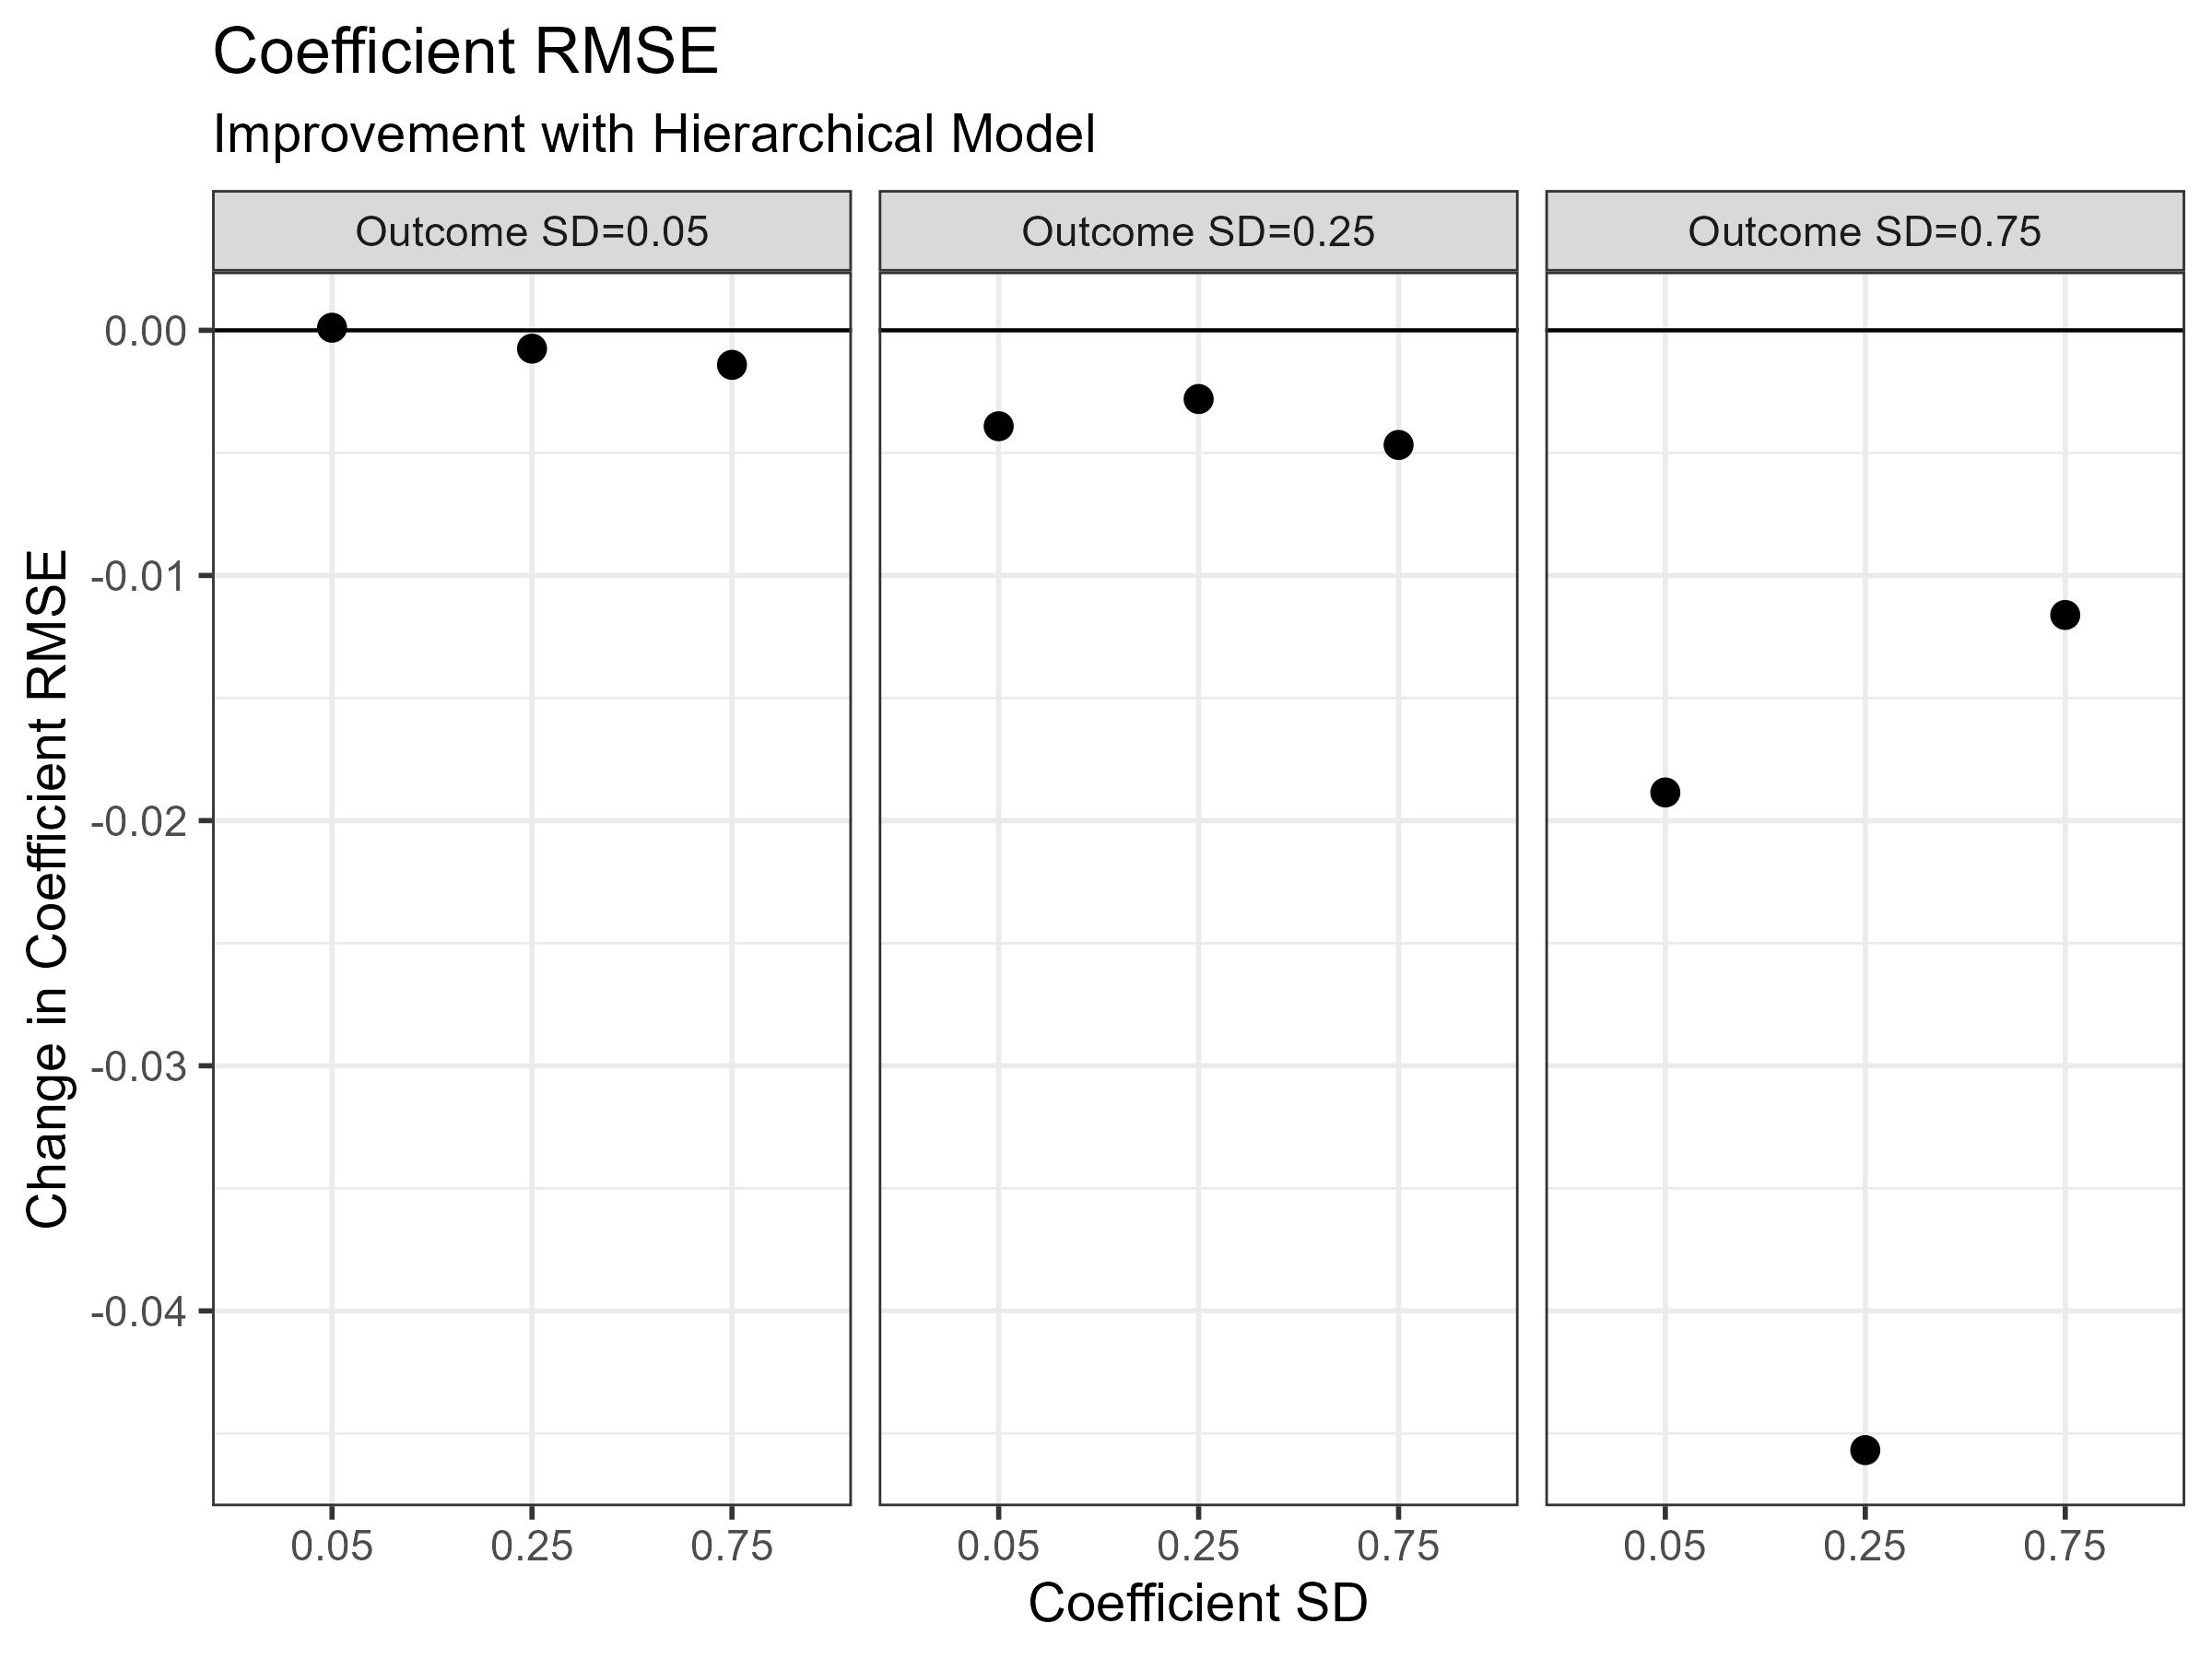
\includegraphics[width=0.95\textwidth]{../figures/sim-rmse-coef-nsd.png}
	\caption{Difference in root mean squared error between hierarchical and OLS estimators of heterogeneous effects with different levels of random variation in the heterogeneous effects and outcome. Positive values favor OLS, and negative values favor hierarchical modeling. Simulations based on 1,000 observations with 32 unique groups.}
	\label{fig:sim-rmse-coef-nsd}
\end{figure}


When the outcome has low variance, OLS and hierarchical models perform similarly. 
This implies that regularization is most important when the outcome is noisy. 
Hierarchical models offer slight improvements at the next highest level of outcome variance, regardless of how much variance there is in the coefficients themselves. 
Hierarchical modeling produces the largest gains at the highest levels of outcome variance, especially when the coefficients vary less than the outcome.
As is often the case, the regularization benefits of hierarchical modeling are greatest when there is substantial noise in the data-generating process. 
OLS estimates of heterogeneous effects are more sensitive to random variation in the outcome.


In the second simulation, I define between 2 and 6 groups in a dataset with 1,000 observations.
Each group has the same number of data points, so as the number of groups increases, the number of observations in each group falls. 
More and smaller groups will likely benefit more from regularization, improving the performance of hierarchical modeling.


\autoref{fig:sim-rmse-coef} summarizes the results of the second simulation.
Again, this figure plots the difference in root mean squared error between the hierarchical and OLS estimators, and negative values mean that the hierarchical models performs better.
Because the number of observations is fixed, as the number of grouping variables rises, the size of the groups falls. 
For instance, with two grouping variables, there are 250 observations per group.
With seven grouping variables, there are 7 or 8 observations per group.


\begin{figure}[htpb]
	\centering
		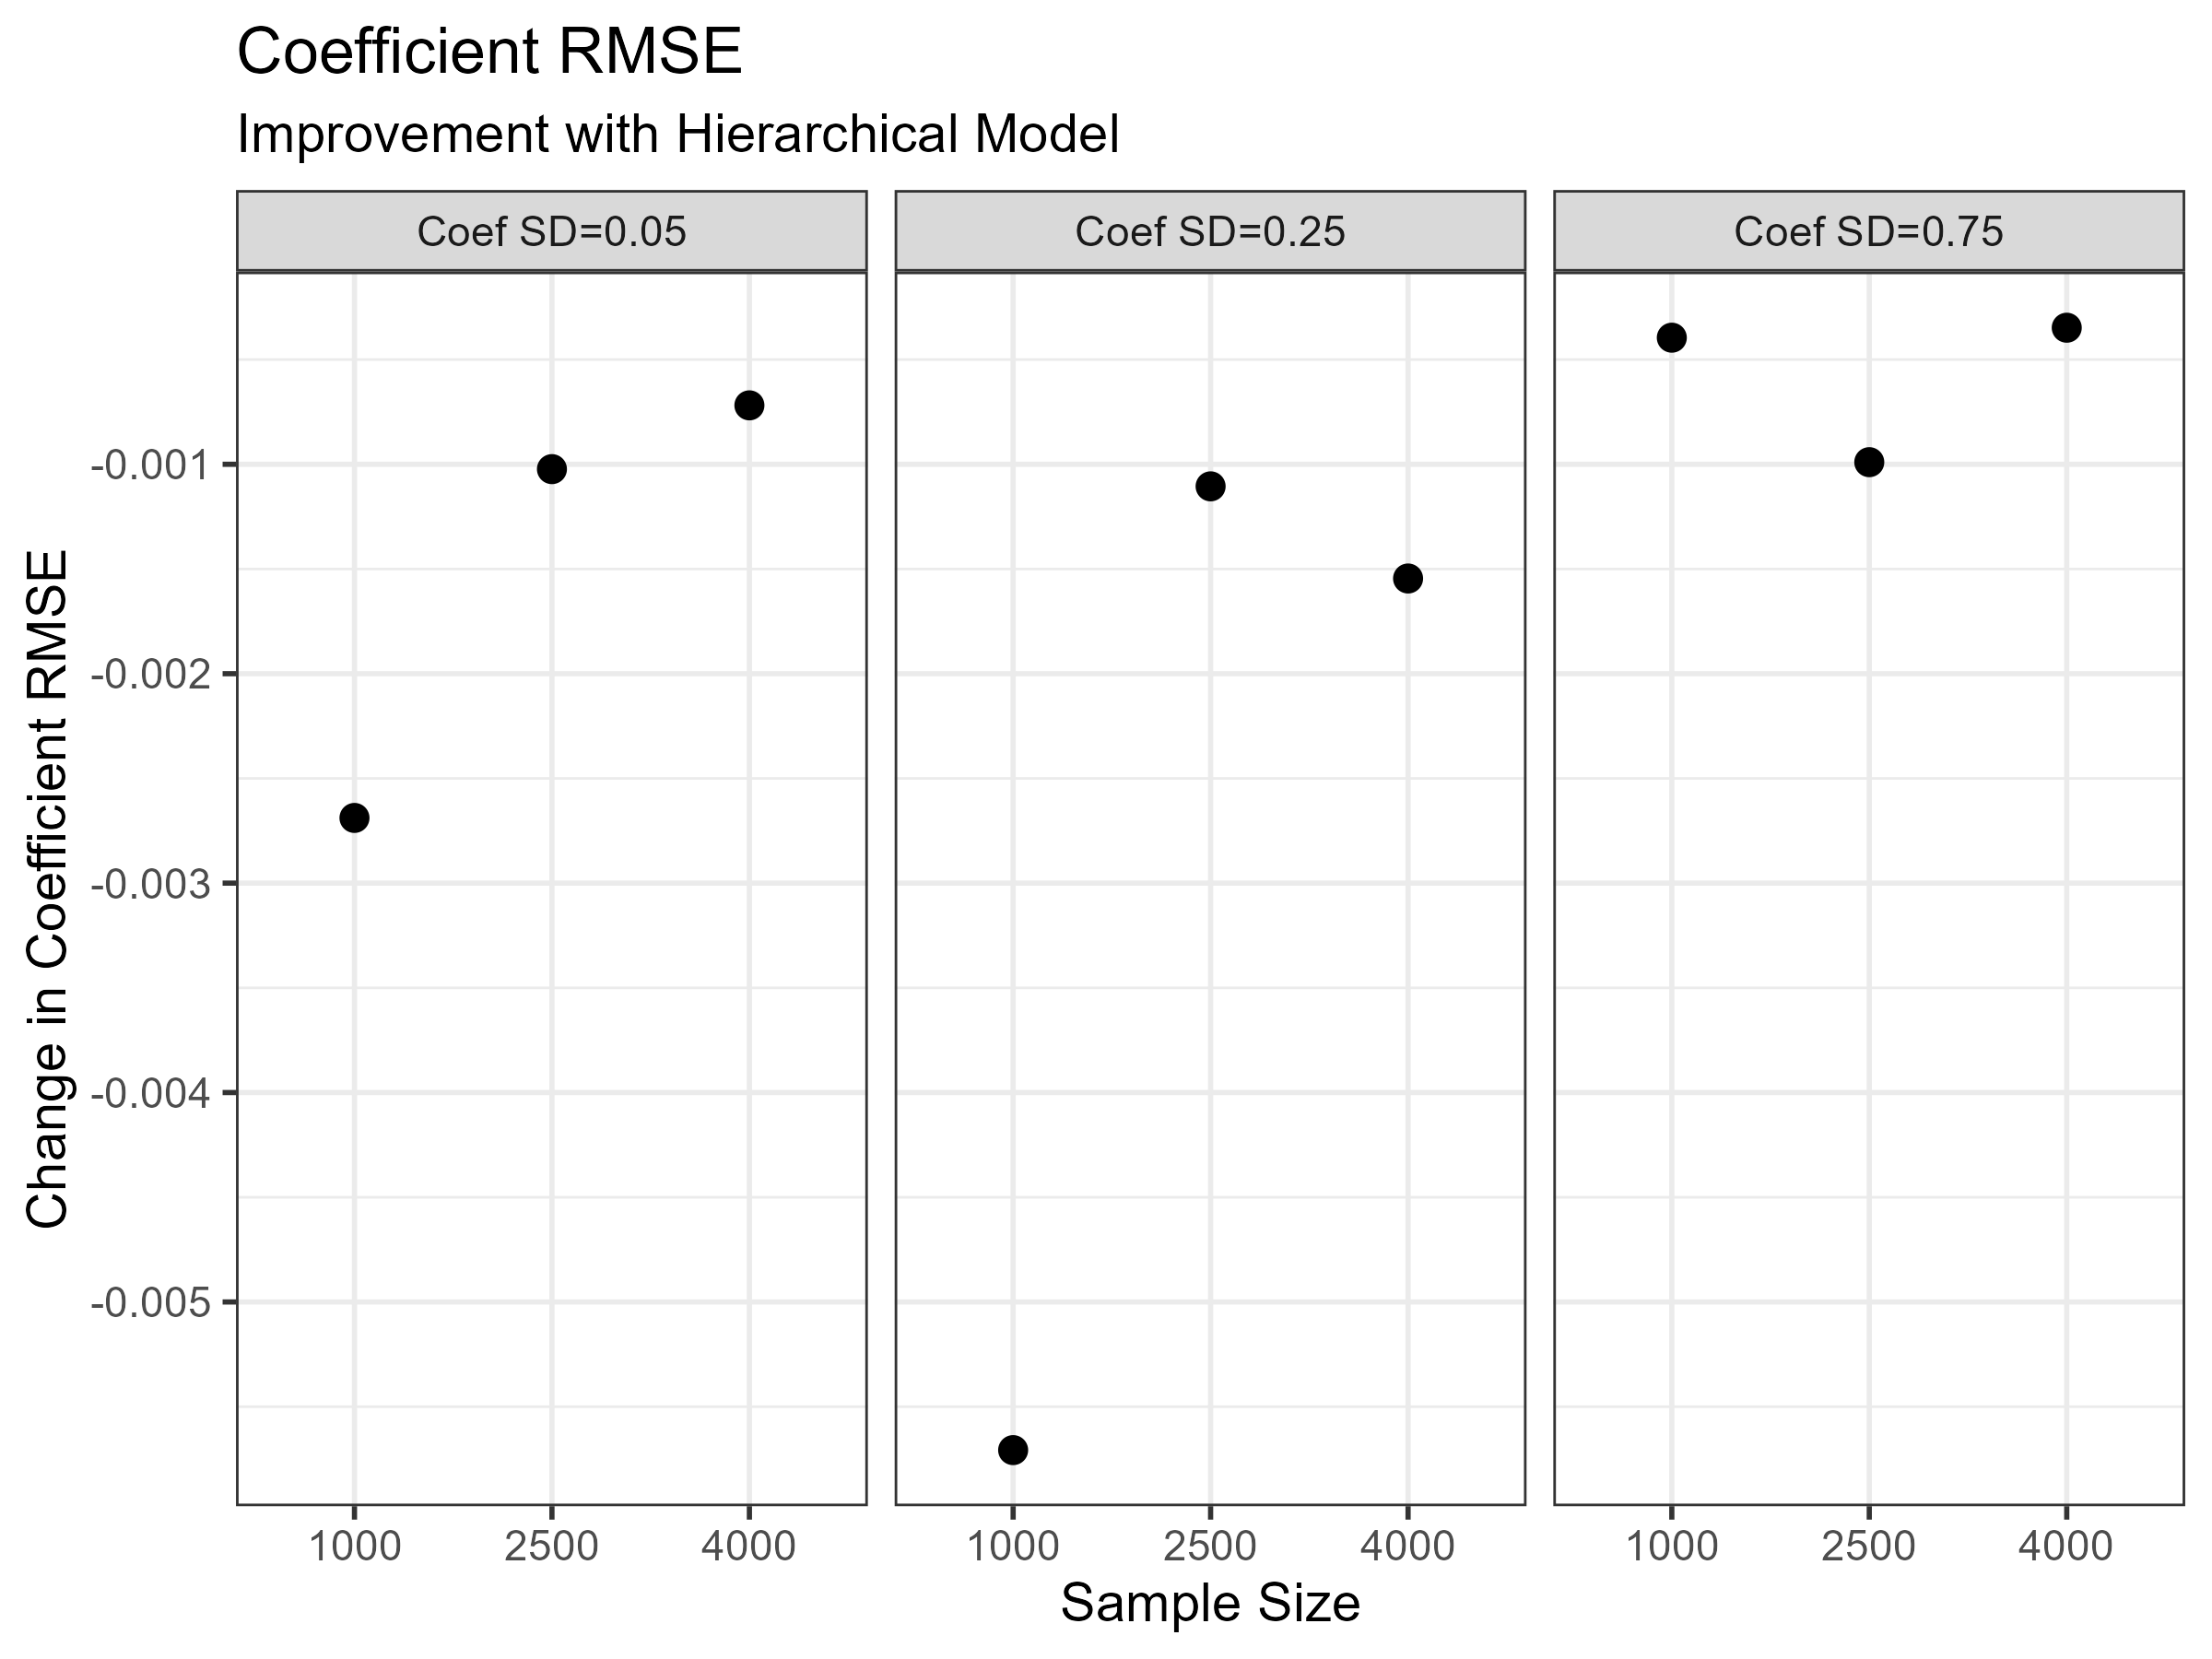
\includegraphics[width=0.95\textwidth]{../figures/sim-rmse-coef.png}
	\caption{Difference in root mean squared error between hierarchical and OLS estimators of heterogeneous effects with different levels of random variation in the heterogeneous effects and outcome as well as different numbers of grouping variables. Positive values favor OLS, and negative values favor hierarchical modeling. Simulations based on 1,000 observations.}
	\label{fig:sim-rmse-coef}
\end{figure}





\section{Example Application: Alliances and Public Support for War} 


In the following, I further demonstrate how the hierarchical approach works and the benefits of regularizing effect estimates by reanalyzing a study by \citet{TomzWeeks2021}. 
Tomz and Weeks (TW hereafter) examine whether the public is more willing to go to war for an allied country.
In a factorial experiment with vignettes, they find a 33\% average increase in support for military intervention on behalf of another country if that country is an ally. 
This is a large and potentially important relationship, because the United States has a global network of allies. 


Given the size of the main effect, TW's paper is an ideal scenario for comparing interactions and hierarchical models. 
Corresponding interaction effects may be large, and their sample size of 1,200 respondents is not unusual in published work. 
At the same time, TW estimated an array of interactions to check how other treatments modify the impact of alliances.
There are 64 unique treatment groups with anywhere from 11 to 32 respondents, so estimates of the impact of alliances in the 32 pairs of alliance treatment and control groups employ at most 54 data points. 
As such, employing varying slopes for regularization will likely offer substantial benefits, because the small groups will likely lead to noisy estimates.
I document these gains by analyzing the how other experimental treatments modify the impact of alliances, and then exploring how demographic differences modify the alliance treatment. 



\subsection{Differences by Experimental Scenario}


Along with alliances, TW randomly assign whether the potential beneficiary of U.S. intervention is a democracy or not, the stakes of intervention, the potential costs, and the region of the world. 
They estimate the impact of alliances in the 32 treatment conditions with an OLS model that fully crosses interactions between the treatments, and calculate marginal effects that average over these groups. 
I keep the same fully crossed structure in the treatment interactions to define groups, but use a varying slopes model to estimate the impact of alliances in each treatment group.


\begin{figure}[htpb]
	\centering
		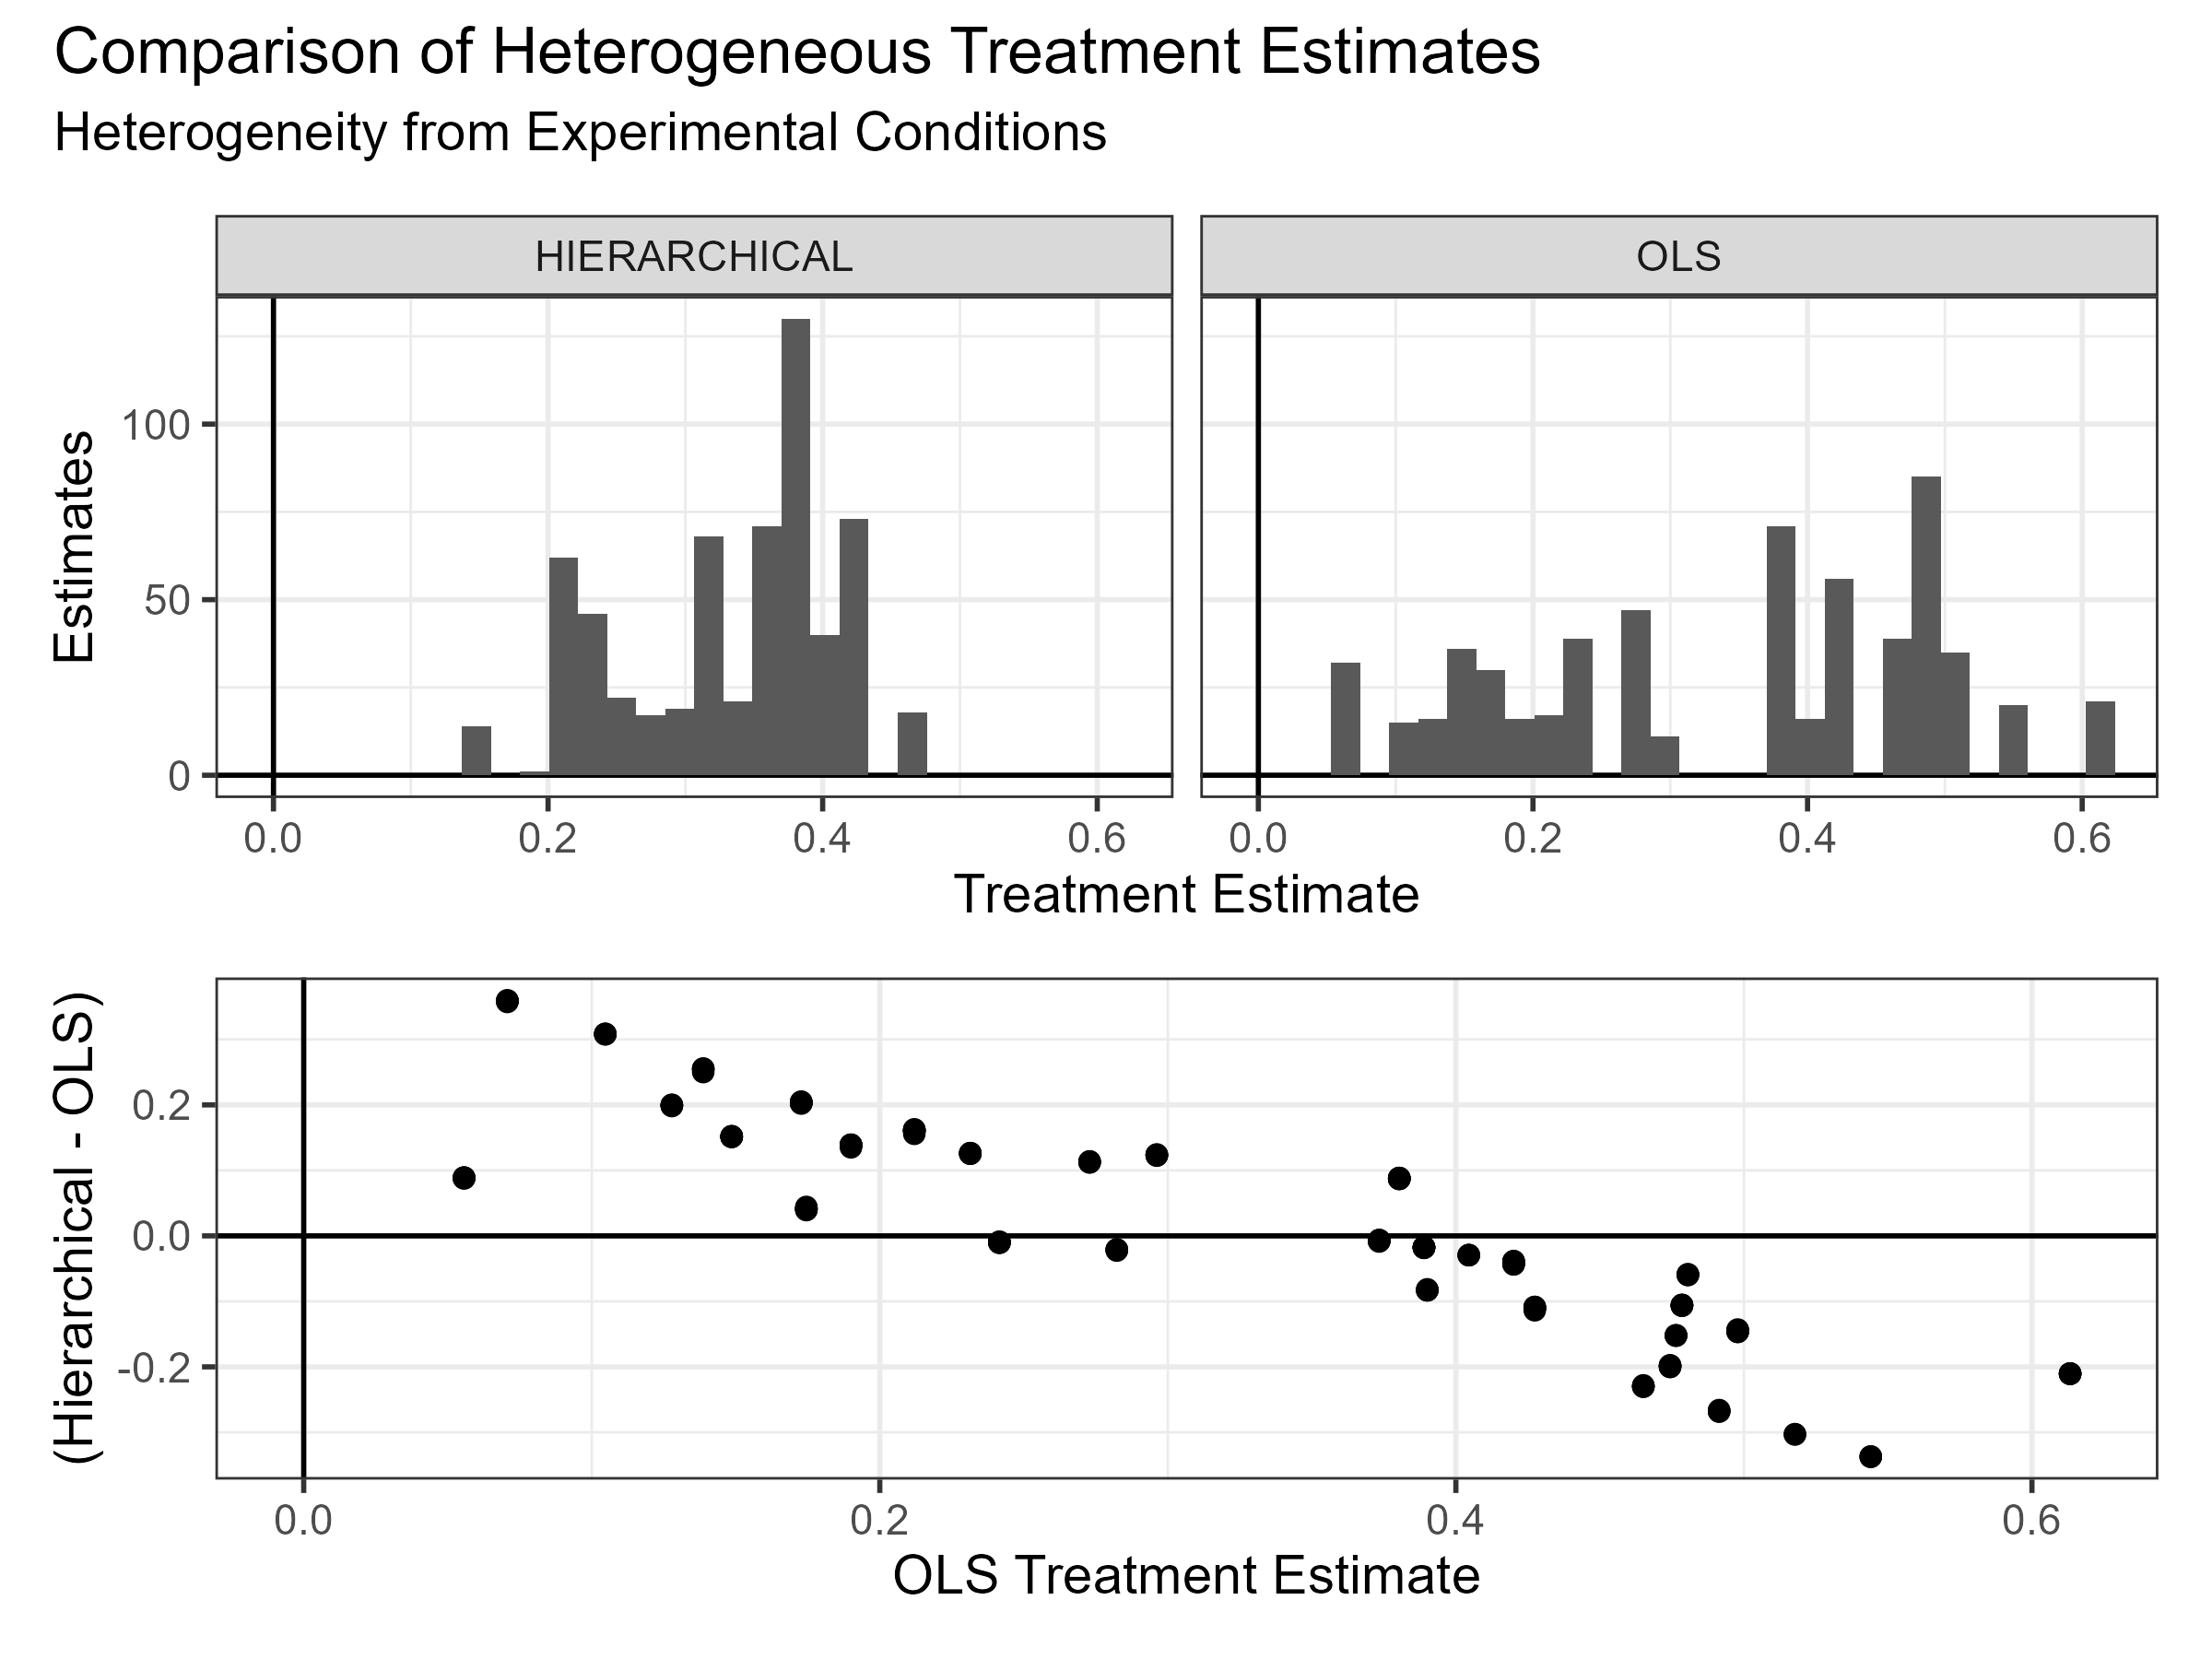
\includegraphics[width=0.95\textwidth]{../figures/tw-het-treat-comp.png}
	\caption{Comparison of OLS and hierarchical estimates of the impact of alliance across experimental conditions. Estimates divided based on the regional treatment variable for ease of presentation. The y-axis is a numeric indicator of the groups, which there are 32 treatment-control comparisons.}
	\label{fig:tw-het-treat-comp}
\end{figure}


\autoref{fig:tw-het-treat-comp} compares the estimated alliance treatment effects across the experimental groups with the OLS and hierarchical models.
Two aspects of \autoref{fig:tw-het-treat-comp} show the regularization benefits of hierarchical modeling.
First, the hierarchical estimates are more precise. 
The credible intervals in the hierarchical model are smaller because they incorporate information from every group. 


Second, the hierarchical estimates are less variable, again due to partial pooling of the slopes.
This reduces the estimated variation in how alliances impact mass attitudes, and is obvious if we compare estimates within regions. 
The OLS interactions are more dispersed, while the hierarchical estimates hew more closely to the overall mean.
This is especially notable in the African and Latin American scenarios. 
Inasmuch as differences across scenarios are driven by noise in small treatment groups, the hierarchical model smooths out some of that random variation.
In some cases, this leads to large shifts in the coefficient estimate.



\subsection{Who Responds to Alliances}


To further explore the potential application of hierarchical models, this section examines how demographic factors modify the impact of alliances.
I used race, gender, hawkishness and internationalism to define demographic groups with fully crossed interactions that produce X number of groups.
I selected these variables because foreign policy dispositions like militant assertiveness shape willingness to use force \citep{Kertzeretal2014} as do gender \citep{Barnhartetal2020} and race. 
I also control for other experimental manipulations.\footnote{See the appendix for priors.} 
Following TW's OLS analysis, I use a Gaussian likelihood, although the outcome is a binary variable. 


I describe the results in three steps. 
First, I summarize the distribution of alliance effects in \autoref{fig:tw-treat-het-sum}. 
After this, I summarize the sources of variation in the alliance effect.
Finally, I compare the hierarchical model with an equivalent OLS specification.

\begin{figure}[htpb]
	\centering
		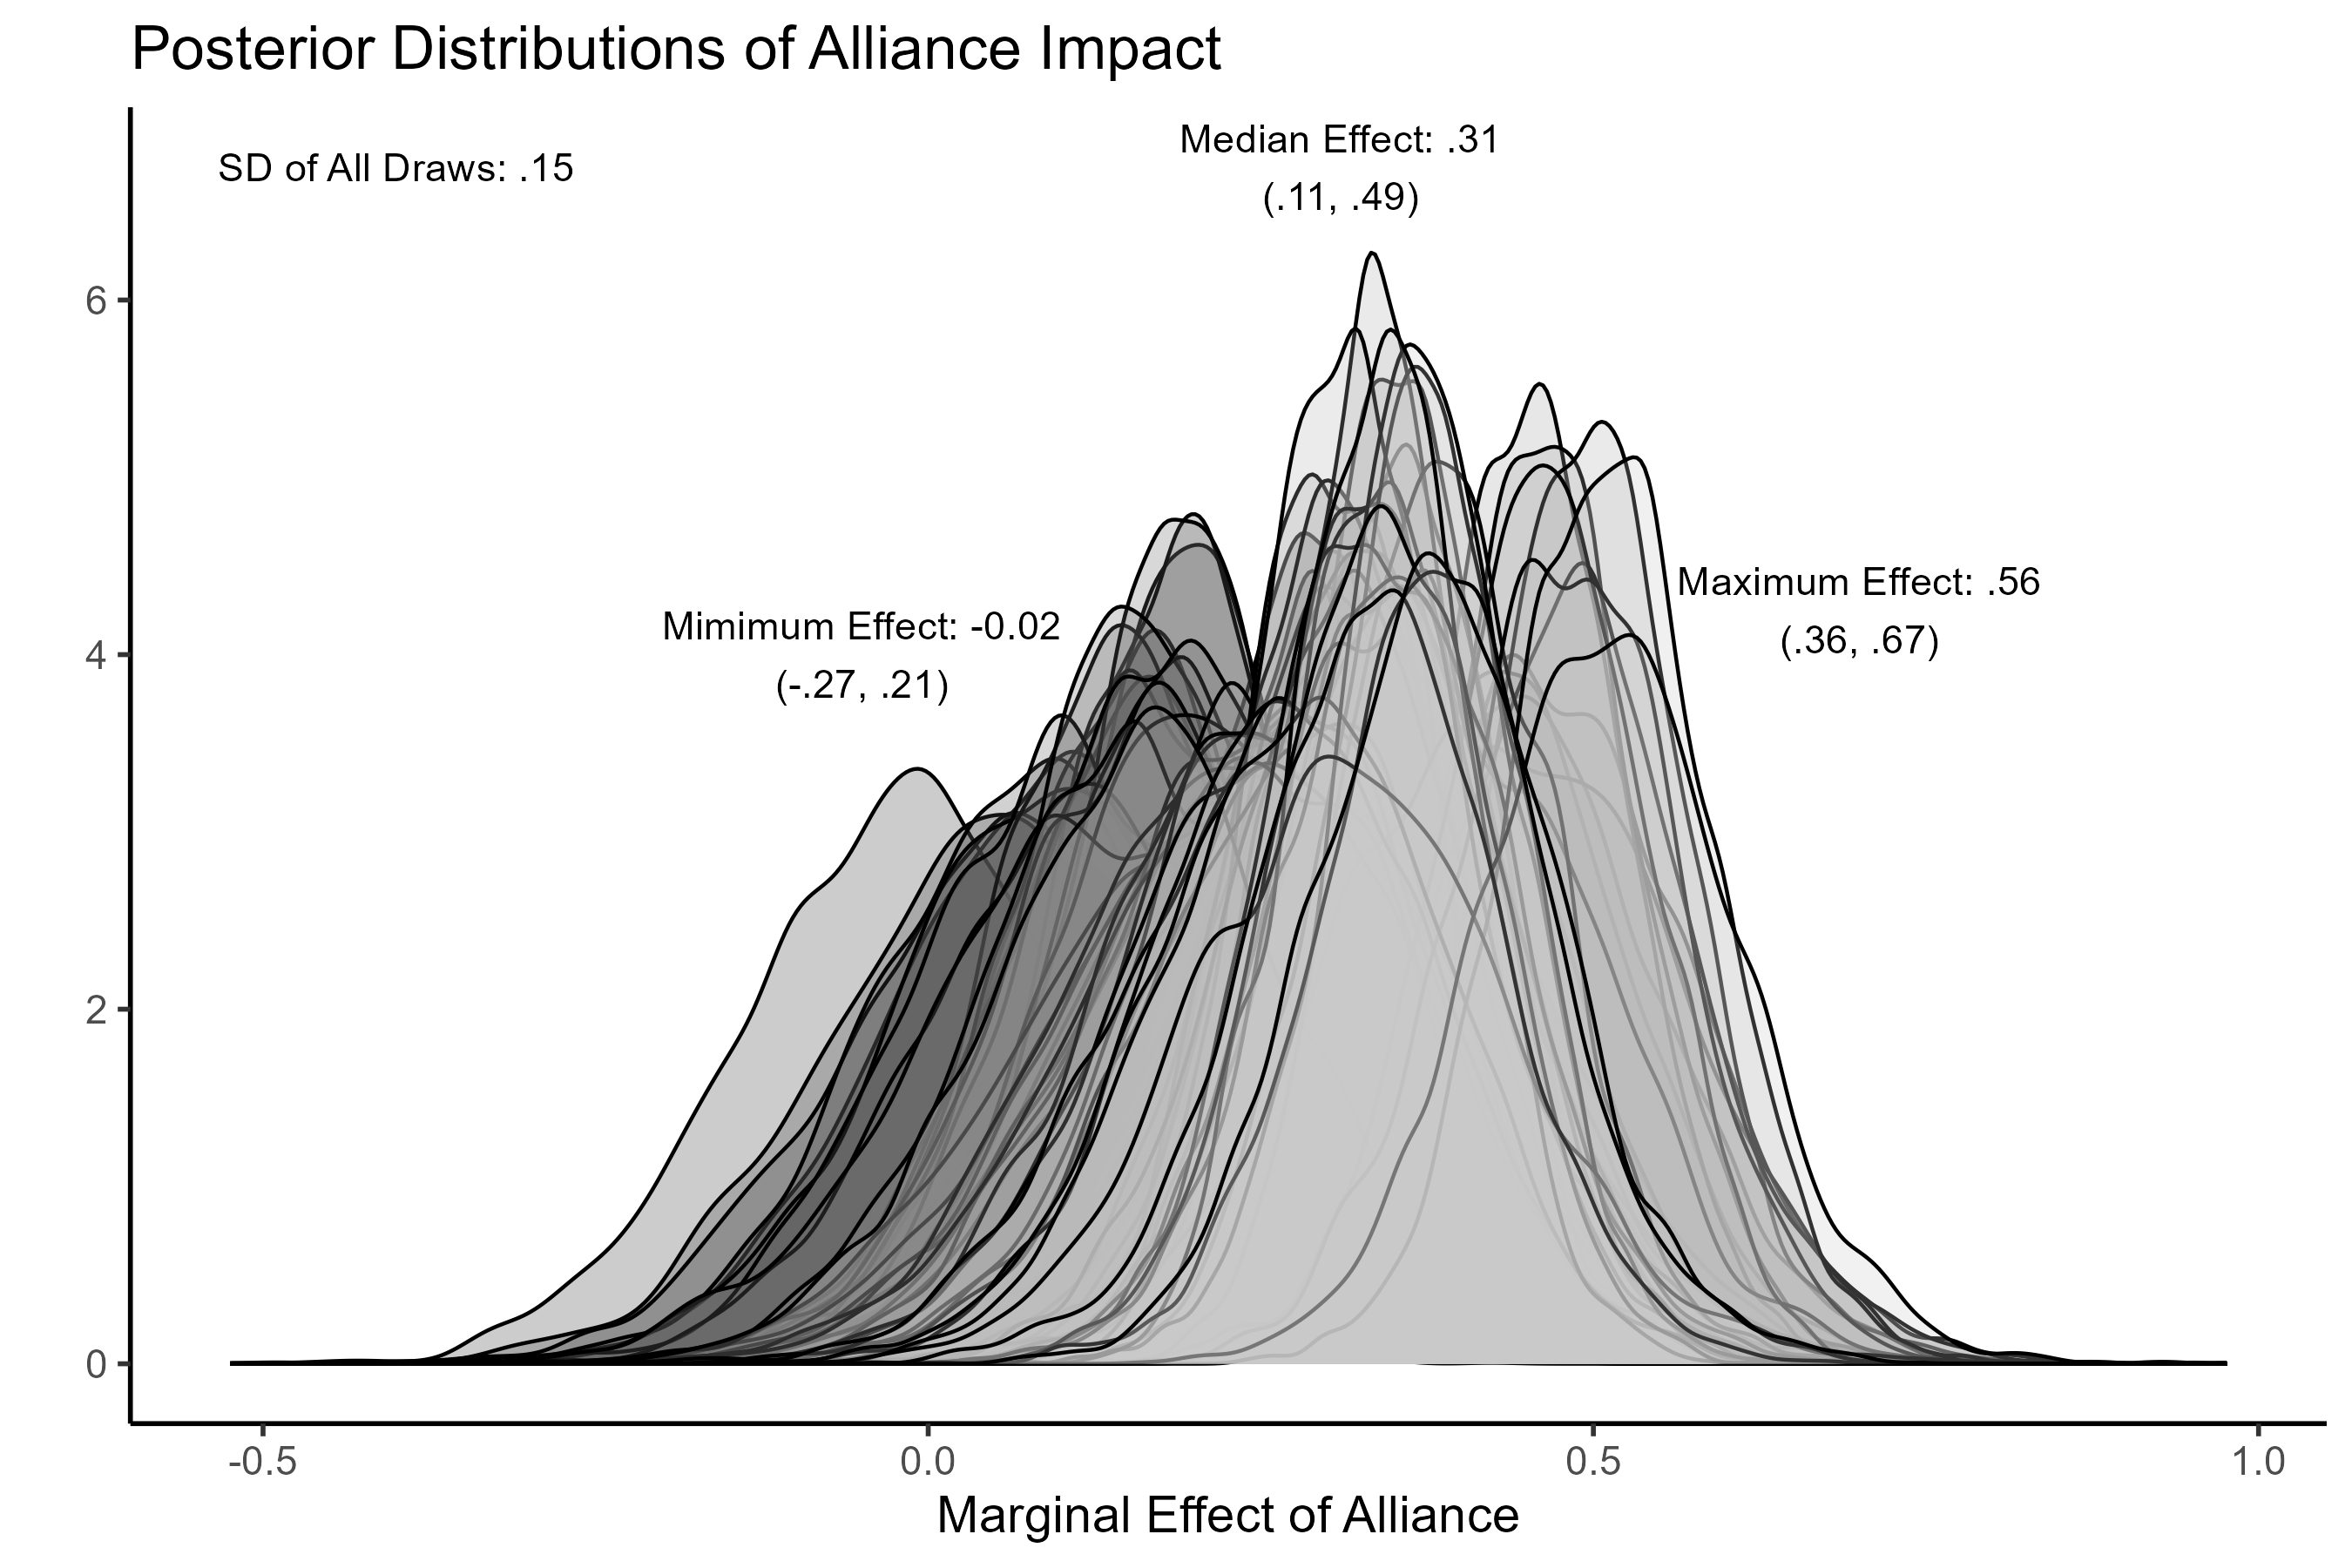
\includegraphics[width=0.95\textwidth]{../figures/tw-treat-het-sum.png}
	\caption{Posterior distribution of all estimated impacts of alliances on support for using force. Text values give notable point estimates, and parentheses summarize the 95\% credible interval.}
	\label{fig:tw-treat-het-sum}
\end{figure}


How alliances impact support for using force varies widely across demographic groups.
\autoref{fig:tw-treat-het-sum} provides an initial summary of that variation, and highlights several noteworthy estimates. 
Key estimates include the median, maximum and minimum effect estimates, as well as the standard deviation of all posterior draws.


First, \autoref{fig:tw-treat-het-sum} notes that the minimum estimated impact of an alliance on a demographic group is -0.08, while the maximum is .53. 
The maximum effect occurs among white men with high internationalism and low hawkishness.
The minimum effect applies to non-white women with low internationalism and high hawkishness. 
There is no overlap in the posteriors of these estimates. 


The median group treatment effect estimate is .31, and this group of respondents is non-white men with middling internationalism and hawkishness. 
This estimate is quite similar to TW's average treatment effect of .33.
That average summarizes enormous demographic differences, however. 
The standard deviation of all posterior draws is .19.


This variation is the result of demographic differences between groups.
\autoref{fig:tw-het-source} plots how the impact of alliances varies across support for international engagement, willingness to use force, race and gender. 
Because there are many groups, the impact of alliances varies widely within each level of these variables, but there are some clear patterns. 


\begin{figure}[htpb]
	\centering
		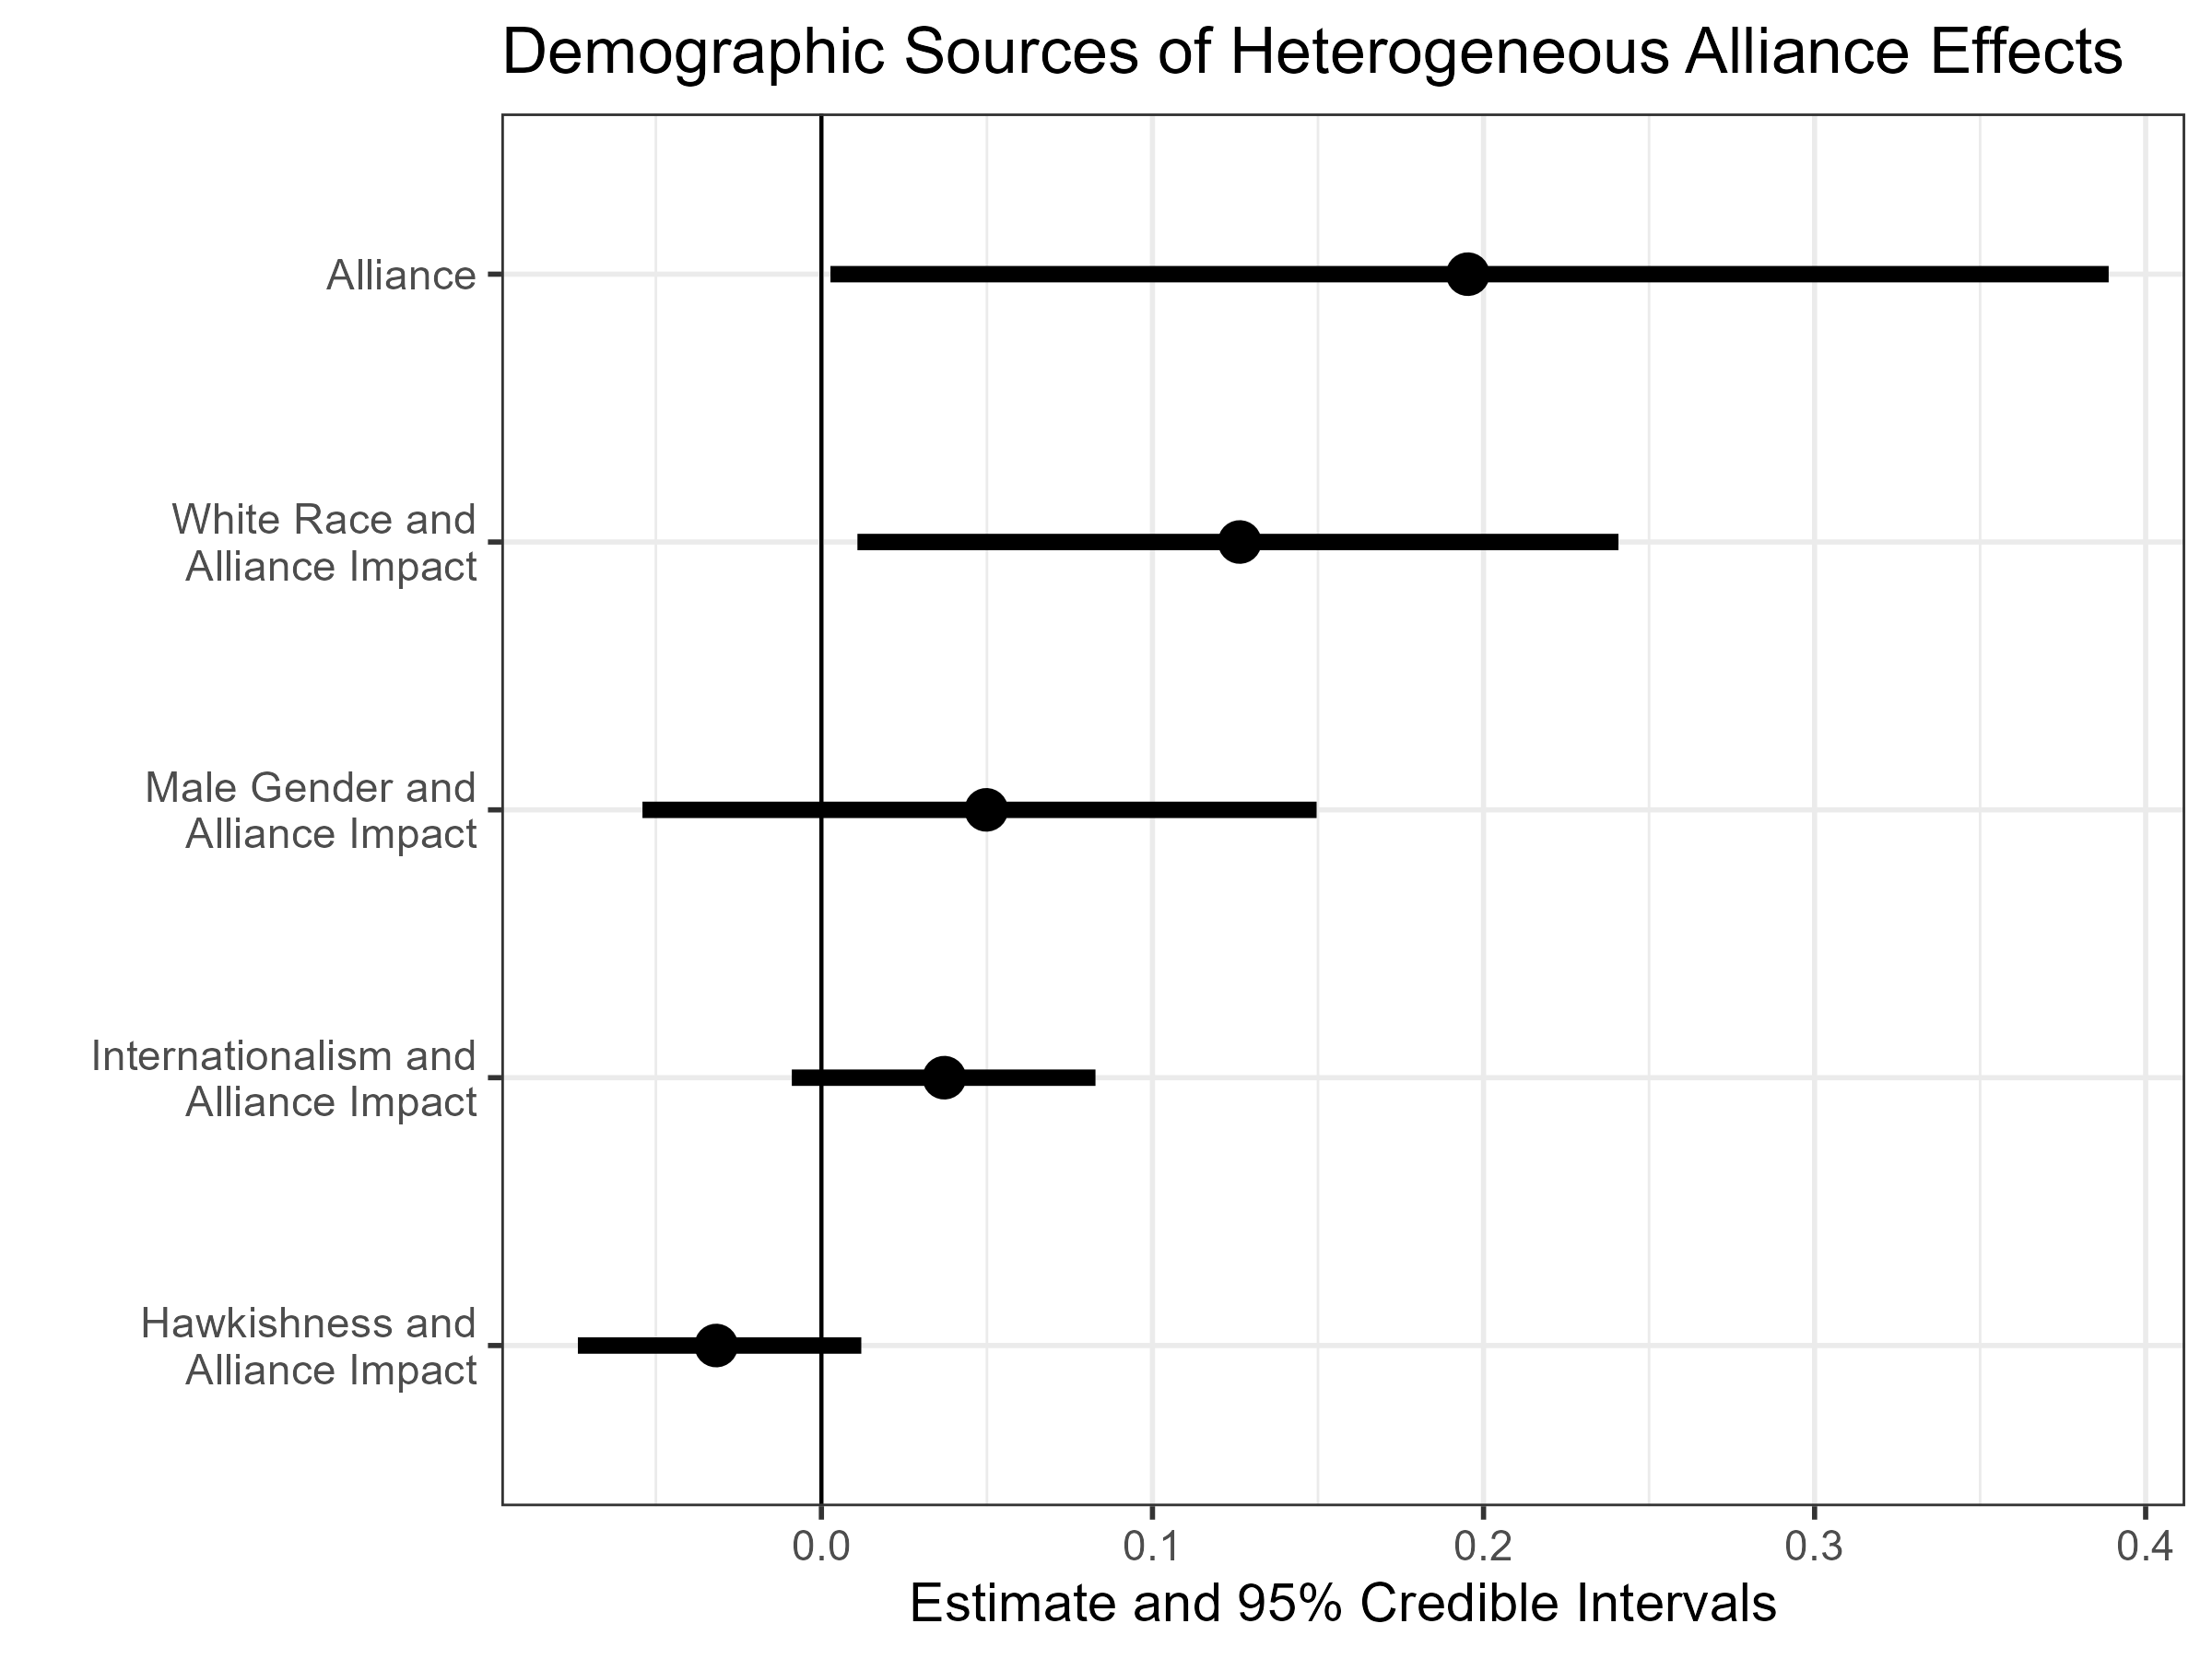
\includegraphics[width=0.95\textwidth]{../figures/tw-het-source.png}
	\caption{Variation in the impact of alliances on support for military intervention across four variables that set groups. Each point marks the impact of alliances on a specific group, and boxplots summarize the median and interquartile range of the slopes within each level of the variable. All slopes are present in each facet.}
	\label{fig:tw-het-source}
\end{figure}


Individuals with minimal interest in international engagement are less responsive to alliances, while any greater support for internationalism leads to a fairly consistent response to alliances. 
Similarly, alliances exert less impact on individuals who have minimal militant assertiveness. 
Alliances are very influential for individuals with low but greater than minimal hawkishness, however. 
Among those with moderate or high hawkishness, alliances have a fairly consistent impact. 
The media alliance impact is also greater for men, and among white respondents. 
Letting slopes vary across each level of the grouping variables generates more flexibility, and clearly shows the difference between individuals with very low internationalism or low militant assertiveness and others. 


As \autoref{fig:tw-het-source} suggests, alliances increase support for foreign intervention most among white men, especially those with low hawkishness and some internationalism.
By contrast, alliances have little impact on support for war among non-white females who are also skeptical of international engagement and unwilling to use force.
Individuals with more ambivalent foreign policy views respond more typically to TW's alliance treatment. 


All these estimates suggest that internationalism matters more than than hawkishness for understanding who is willing to fight for U.S. allies. 
Alliances may impact hawks less because these individuals support intervention regardless. 
Military alliances matter most to backers of international engagement who less willing to use force, but not entirely averse to military intervention.

\begin{figure}[htpb]
	\centering
		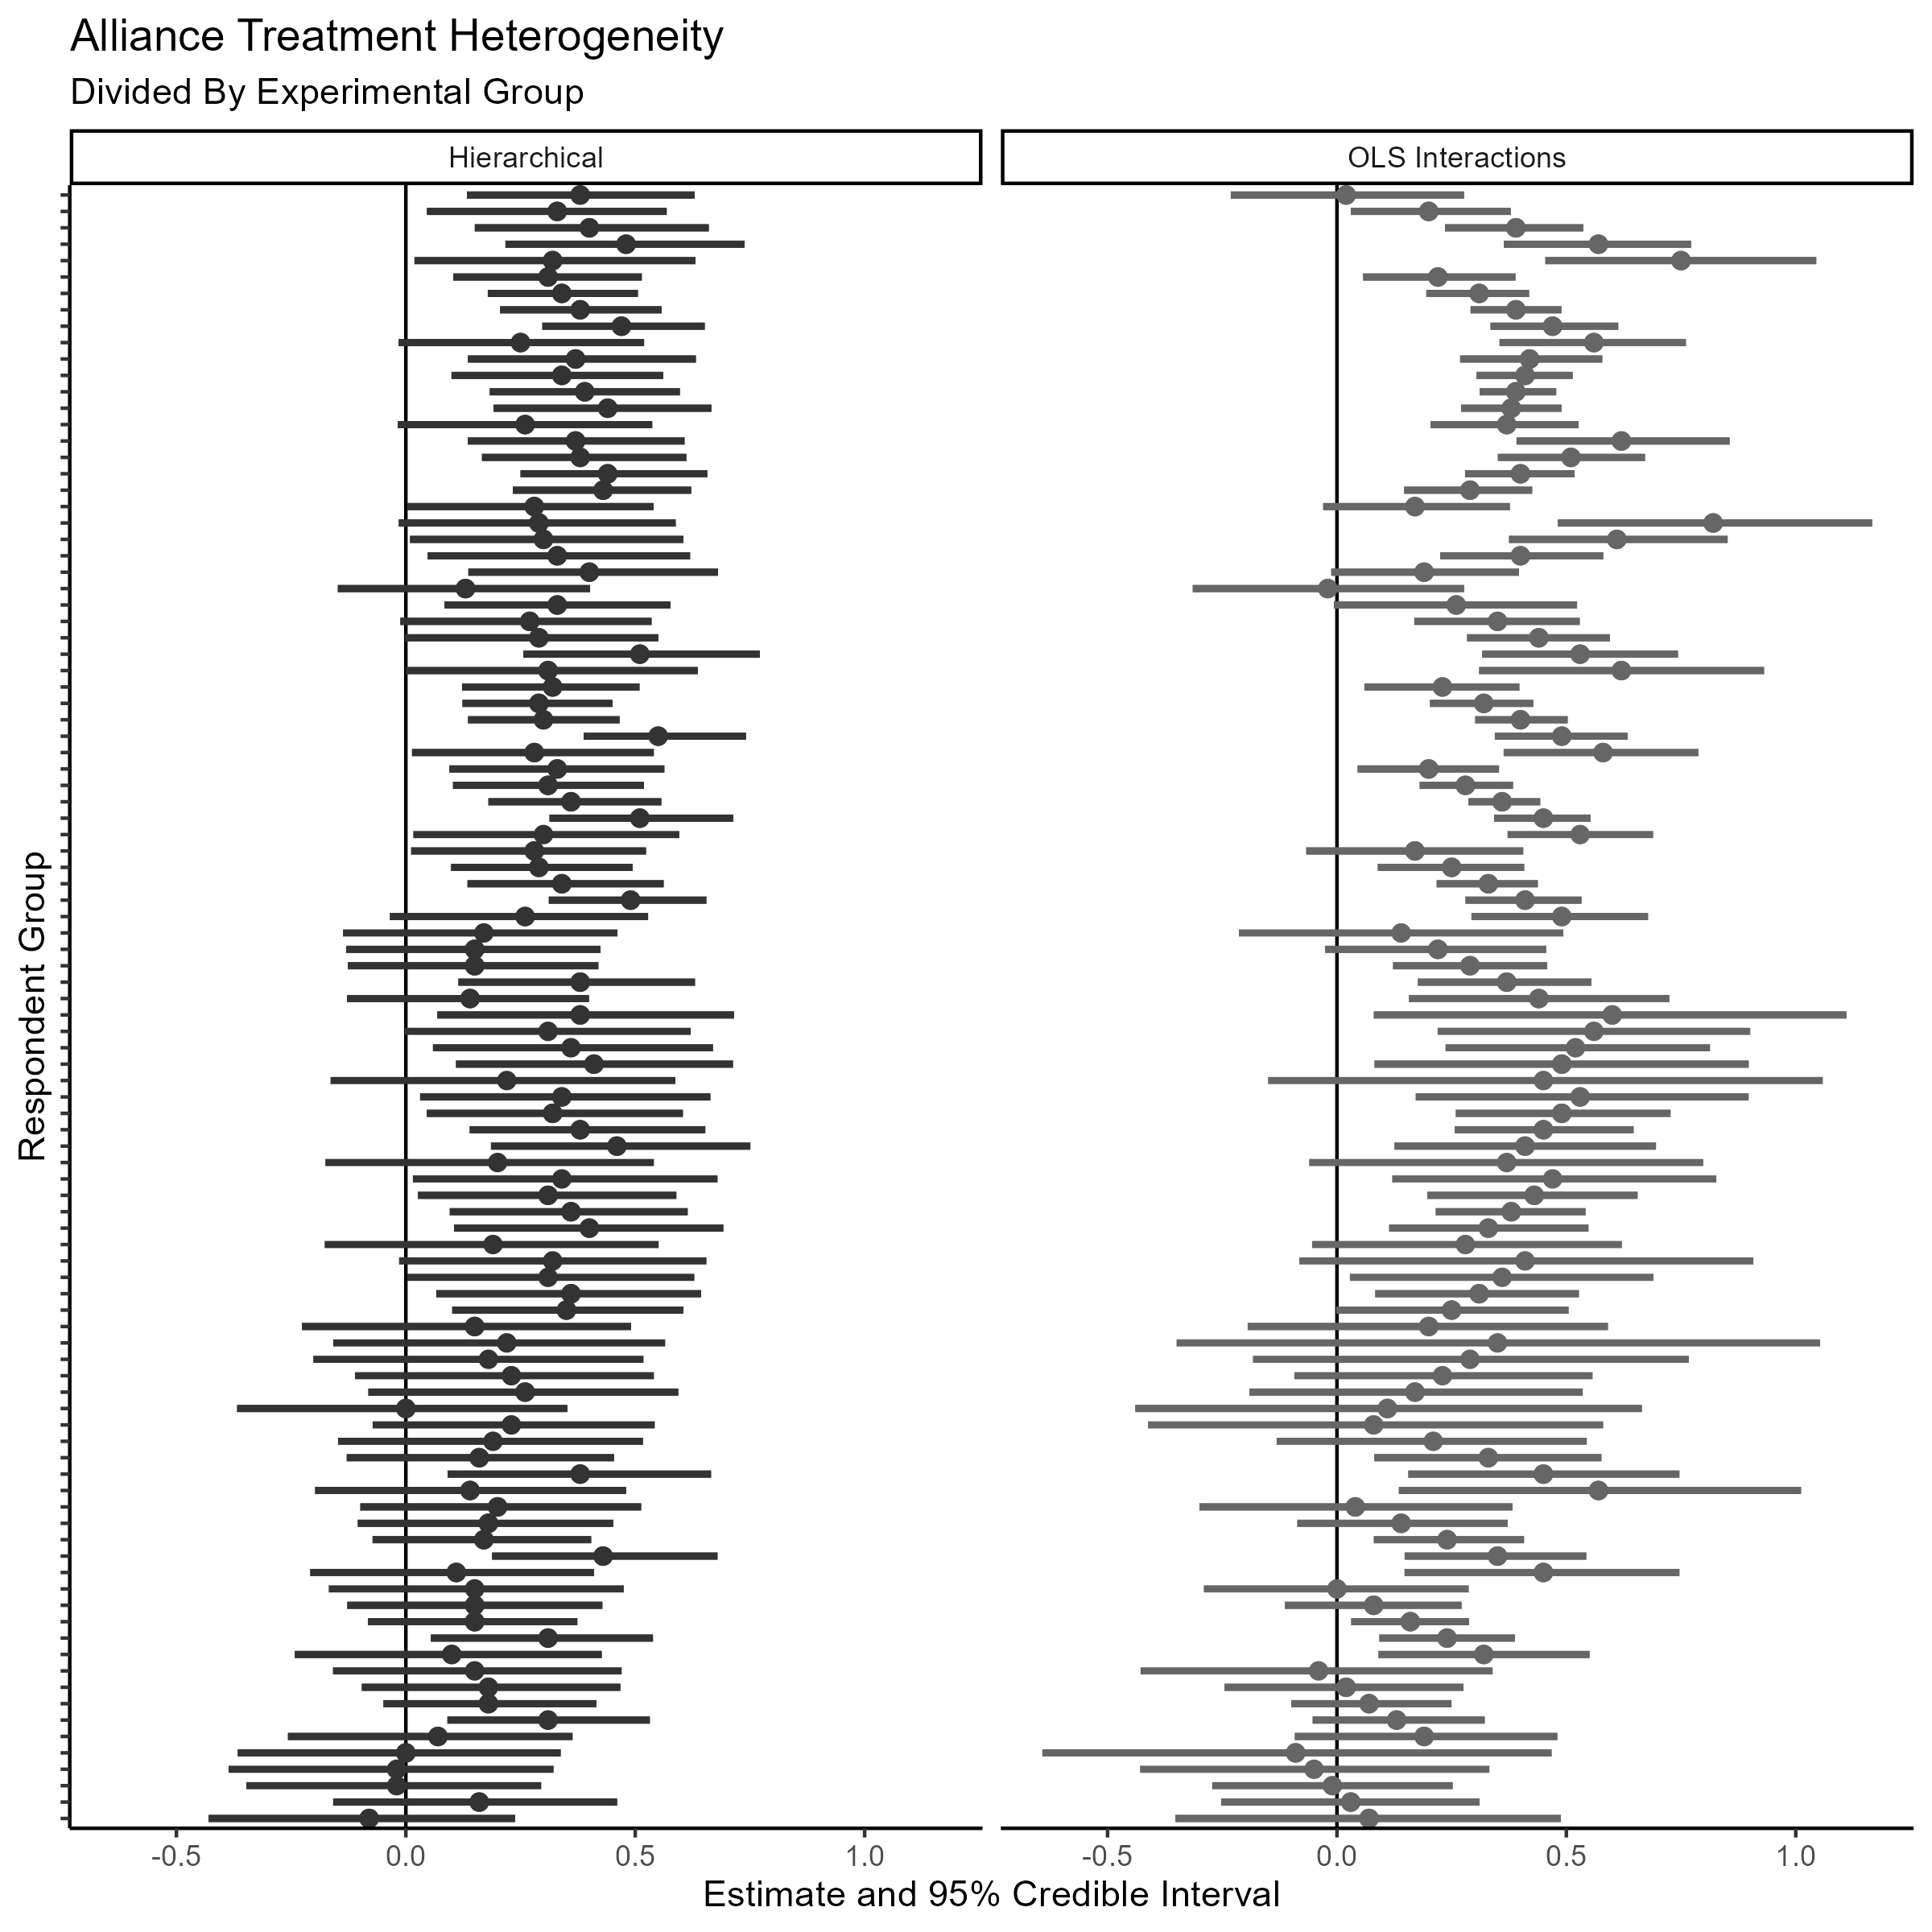
\includegraphics[width=0.95\textwidth]{../figures/tw-treat-het-comp.png}
	\caption{Estimated impact of alliance on support for military intervention in different subgroups of respondents. Groups defined based on fully crossed interactions between the demographic variables. Error bars give the 95\% credible interval in the hierarchical model and 95\% confidence interval in the OLS interactions model.}
	\label{fig:tw-demog-comp}
\end{figure}


Finally, I illustrate the regularization benefits of a hierarchical model in \autoref{fig:tw-demog-comp}.
Again, the hierarchical estimates are more precise and less variable than OLS with fully crossed interactions. 
This occurs because the model partially pools information across groups, which reduces uncertainty and pulls the estimated alliance impact towards the overall mean.


The other noteworthy concern is that OLS estimation with fully crossed interactions can make strong extrapolations.
In some groups, the estimated impact of an alliance rises to 80 or 90\%. 
This is the result of the purely linear estimation in OLS that stacks additive terms.
Hierarchical models somewhat relax this, and are less likely to pick up noise in the data.


% variation
These results show some of the strengths and weaknesses of the hierarchical approach to heterogeneous effects.\footnote{In the appendix, I analyze \citet{BushPrather2020}.}
A simple model based on demographic groups provides precise insights about who heeds alliances in supporting using force abroad. 
At the same time, because some demographic groups are small and the model pulls groups towards the overall mean, powerful comparisons between most groups is challenging. 
Fewer groups would have more data and less uncertainty but perhaps obscure variation across key demographic characteristics. 


\section{Conclusion}


This note explained how and when to use hierarchical models to estimate heterogeneous effects. 
Bayesian modeling can apply to a wide range of outcomes, data structures, and theories. 
It also details what drives variation in an effect and how much an effect varies. 
Explicitly modeling how different groups respond to an independent variable can help test arguments and inform policy.  


Hierarchical modeling provides an intermediate approach between interactions or subgroup analyses and machine learning algorithms. 
For interactions with one or two variables, relying on simple interaction tools is best. 
Similarly, machine learning is best for discovery of complex heterogeneity.
When there are two or more modifiers and many groups of theoretical interest, hierarchical modeling allows theoretically informed and interpretable estimation of effect variation. 

As a result, hierarchical modeling complements existing tools and should not replace them. 
Researchers can use hierarchical models to check and inform other techniques, for instance by seeing if a key interaction holds when there are multiple modifiers, or comparing multiple modifiers that past theories have identified. 
Using hierarchical modeling can thus help scholars and policymakers better understand heterogeneous effects.


\section*{Acknowledgements}

Thanks to Taylor Kinsley Chewning, Andrew Gelman and Carlisle Rainey for helpful comments.

\singlespace
\bibliography{../../MasterBibliography} 


%\documentclass[12pt]{article}

\usepackage{fullpage}
\usepackage{graphicx, rotating, booktabs} 
\usepackage{times}
\usepackage{fbb} 
\usepackage{natbib} 
\usepackage{indentfirst} 
\usepackage{setspace}
\usepackage{grffile} 
\usepackage{hyperref}
\usepackage{adjustbox}
\usepackage{multirow} 
\usepackage{amsmath}
\usepackage[labelfont={bf},textfont=it,labelsep=period]{caption}
\setcitestyle{aysep{}}
\usepackage{sectsty}
% for the big table
\usepackage{afterpage}
\usepackage{array}
\usepackage{lscape}
\usepackage{longtable}
\usepackage{float}
\sectionfont{\Large}
\subsectionfont{\noindent\large\textit}
\subsubsectionfont{\normalsize}


\singlespace
\title{\textbf{Appendix: Using Hierarchical Models to Estimate Heterogeneous Effects}}

\date{}
\bibliographystyle{apsr}

\begin{document}


\maketitle 

\singlespace 

\tableofcontents



\section{Tomz and Weeks Reanalysis}

This summarizes a heterogeneous treatments model of \citep{TomzWeeks2021} and details the underlying \textsf{R} code. 

\subsection{Heterogeneous Treatments} 

Here, I examine how the impact of alliances varies with other factors in the experiment, especially costs, stakes, region and partner democracy.
The heterogeneous treatment model corroborates TW's conclusion that alliances exert the greatest impact in instances when public opinion is otherwise skeptical of intervention.

\autoref{fig:tw-het-treat} supports TW's findings that alliances exert the most influence in situations where the public is otherwise unlikely to intervene. 
This figure shows the impact of alliances in unique combinations of all other experimental treatments. 
For a hypothetical democracy in Eastern Europe where intervention has high stakes, alliances exert minimal impact on public attitudes. 
In low-stakes and high cost interventions to support African, Asian or Latin American dictators, alliances increase support for intervention by 50\%. 
Beyond these systematic differences, random variation that is not attributed to the other treatments is roughly 6\%. 


\begin{figure}[htpb]
	\centering
		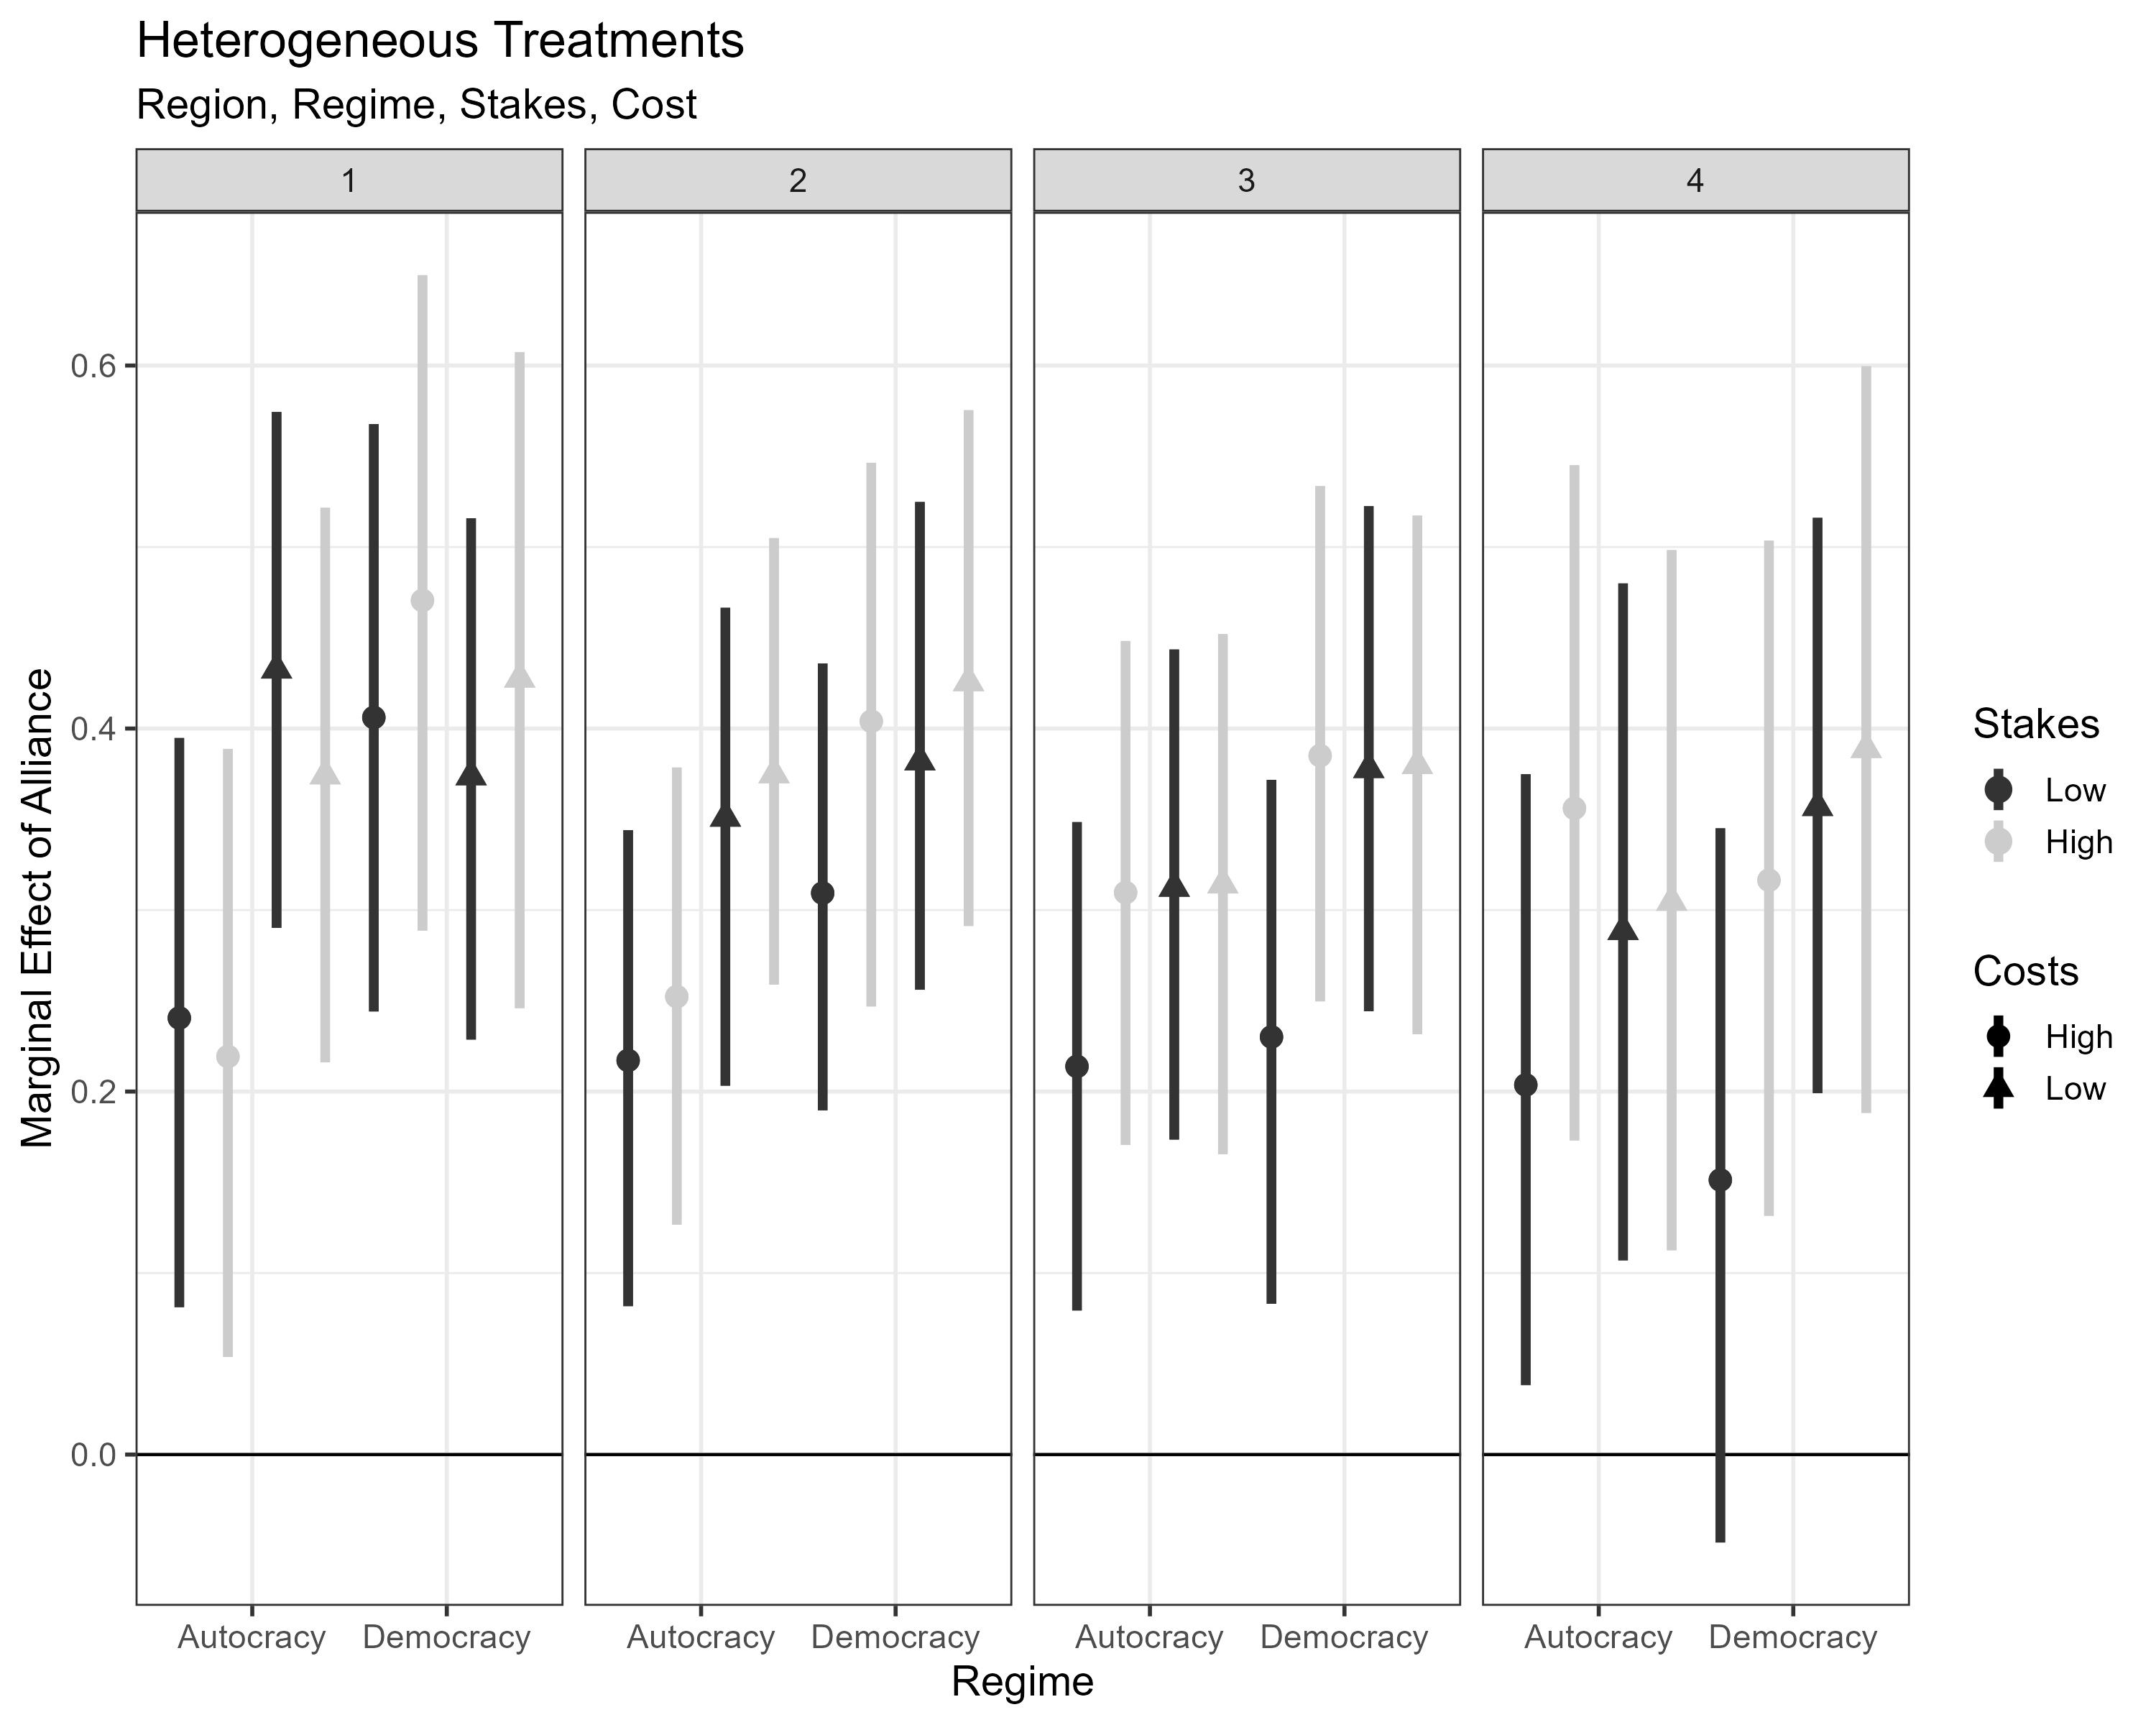
\includegraphics[width=0.95\textwidth]{tw-het-treat.png}
	\caption{Estimated impact of military alliances on public support for war across hypothetical region, costs, stakes and partner regime. Colors distinguish stakes, point shapes mark different costs, and estimates are grouped by regime type. Point estimates give the posterior median and error bars summarize the 95\% credible interval.}
	\label{fig:tw-het-treat}
\end{figure}


\subsection{R Code: Tomz and Weeks Reanalysis}

First, the following model formula expresses a heterogeneous treatments model where the impact of alliances varies with the regime under attack, the stakes, the costs, and the region. 
The \verb+treat.group+ indicator marks unique combinations of the regime, stakes, costs and region variables. 
It can also be written as \verb+regime:stakes:costs:region.txt+. 
I also control for gender, race, and three foreign policy dispositions. 

\begin{verbatim}
bf(force ~ 1 + white + male + hawk + intl + natl.sup + 
             alliance*(regime + stakes + costs + region.txt) + 
             (1 + alliance | treat.group) 
\end{verbatim}


The second formula expresses a treatment heterogeneity model where the impact of alliances varies with gender, race, and three foreign policy dispositions. 
The \verb+het.group+ indicator marks unique combinations of the demographic modifiers.
It can also be written as \verb+white:male:intl:hawk+. 
In this model, the other experimental conditions are controls. 

\begin{verbatim}
bf(force ~ 1 + regime + stakes + costs + region.txt +
             alliance*(white + male + intl + hawk) +
             (1 + alliance | het.group) 
\end{verbatim}



\section{Bush and Prather Reanalysis}


In the following, I again demonstrate how the model works by reanalyzing a study by \citet{BushPrather2020} (BP hereafter). 
This study examines how foreign meddling in elections impacts support for economic engagement with the meddler. 
One of their experiments examines how Russian or German engagement in the 2016 US election impacts mass support for trade and investment with those countries.
I use a heterogeneous effects model to check their results and further explore their findings. 


% describe design
BP employ a 2x2x2 factorial experiment.
This design randomizes whether a foreign country is interfering in the 2016 election, the country and their attitude towards Trump and whether the potential economic ties entail greater trade or investment in the United States.
In one treatment, Russia expresses support for Trump and in the other, Germany expresses opposition to Trump. 


BP hypothesize that individuals will prefer economic engagement with states that support their candidate. 
They thus examine how the impact of side-taking varies with the direction of the endorsement, individual political preferences, and the economic issue. 
To do this, they use four tables and figures, and rely on eight t-tests of differences in means between groups of roughly 25 respondents. 


The heterogeneous effects model encapsulates the argument and all tests by estimating the impact of side-taking on economic engagement as a function of which country is involved, a dummy indicator of intention to vote for Clinton, and their interaction. 
The interaction captures the hypothesis that Clinton voters will support engagement with Germany because Germany opposed Trump, and should be positive. 
I also add an indicator of whether the experiment deals with trade or investment. 
The heterogeneous effects equation also includes indicators of female gender and political engagement. 
The political engagement measure is a sum of political knowledge and interest. 


The outcome variable is a scale from one to four that measures support for greater economic engagement with the potential partner. 
To approximate BP's analyses, I use a normal outcome likelihood. 
Because this experimental randomization produced a roughly balanced sample, I do not include any control variables in the outcome equation. 


\begin{figure}[htpb]
	\centering
		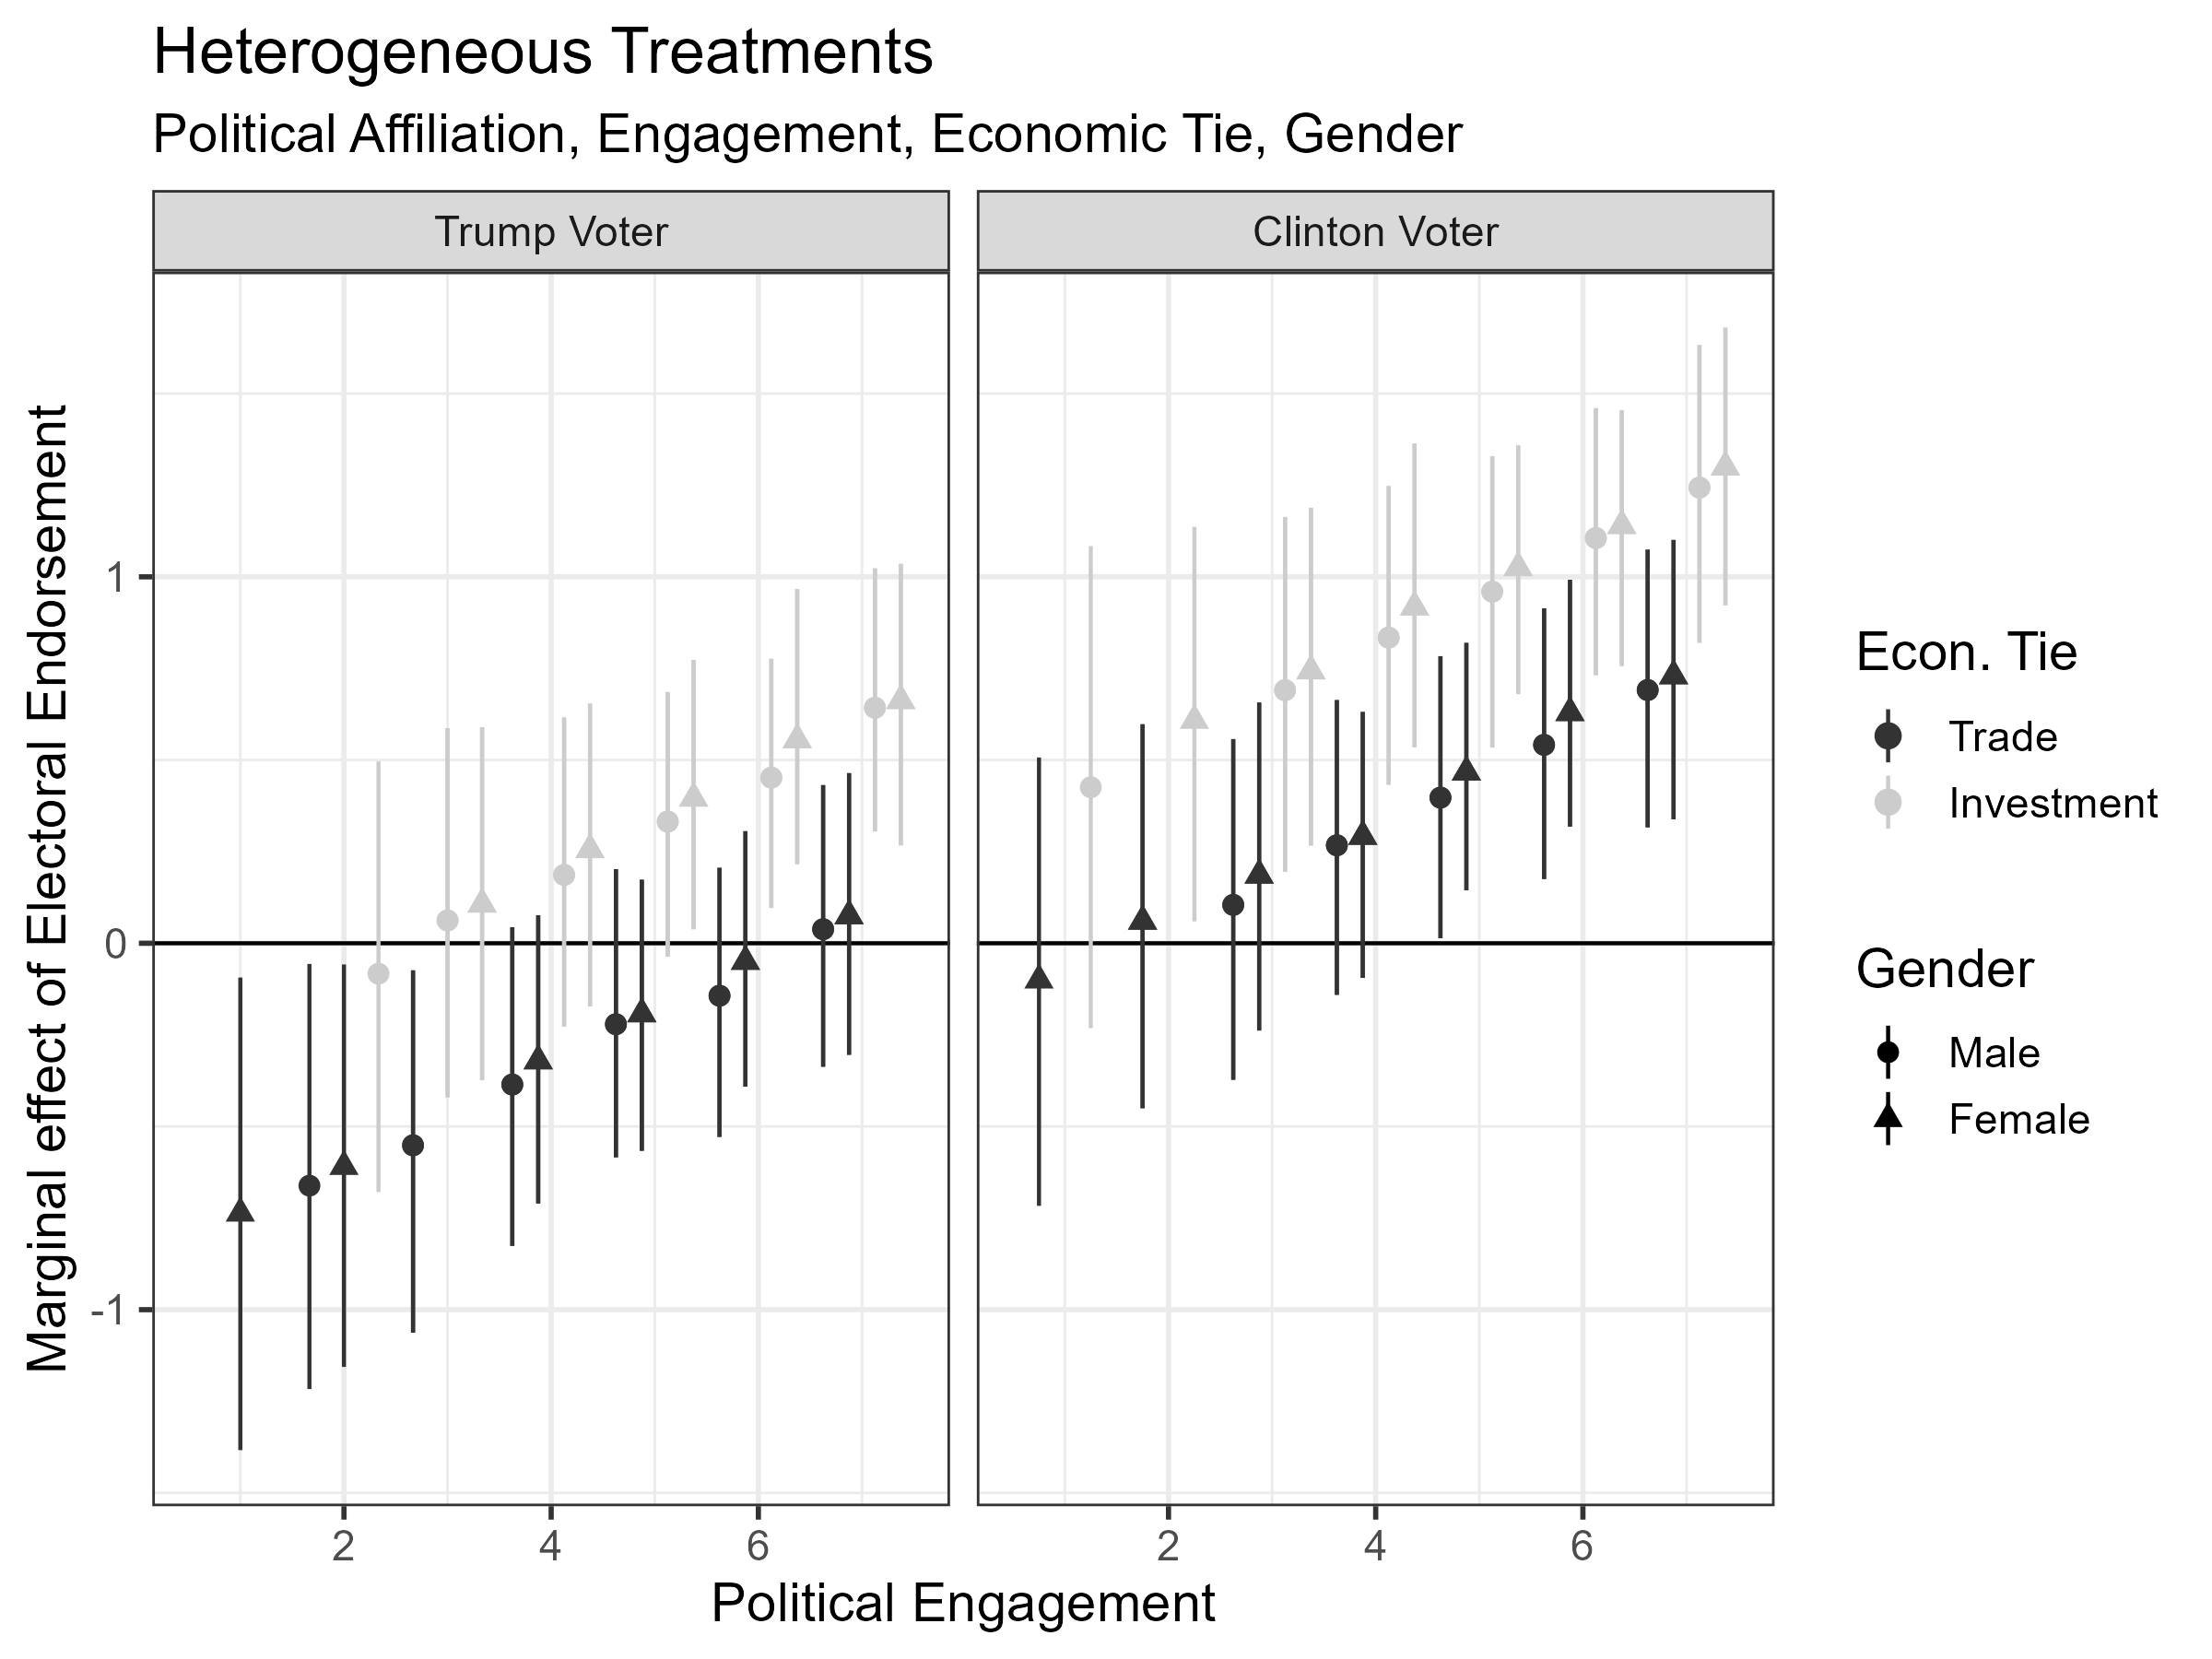
\includegraphics[width=0.95\textwidth]{bp-het-est.png}
	\caption{Heterogeneous effects of German side-taking in US elections on support for economic engagement with Germany. Each estimate reflects a treated group with a unique combination of other treatments and demographic characteristics.}
	\label{fig:bp-het-est}
\end{figure}


These estimates corroborate BP's findings, and also suggest that side-taking exerts the greatest influence on individuals who are highly engaged in politics. 
Clinton voters are more likely to support economic engagement with Germany when Germany has opposed Donald Trump. 
Conversely, some Trump voters oppose greater trade with Germany after the same side-taking. 
The impact of side-taking is also stronger for foreign investment than trade. 
Individuals are more willing to support investment than trade.


Side-taking exerts the most influence on individuals who are highly engaged in politics. 
Engaged Clinton voters respond most to German side-taking against Trump. 
Among these respondents, side-taking increases support for economic engagement by .5 or more, which is a large effect on an outcome that runs from one to four. 


\singlespace
 
\bibliography{../../MasterBibliography} 


\end{document}

\end{document}

